\newcommand{\labtitle}{ECE/CS 5710/6710 - Lab 1}
%\newcommand{\labdate}{September, 4, 2019}
\newcommand{\labsubtitle}{CMOS Inverter - Schematic and Circuit Simulation}
\vlsiheader
	
\begin{center}
	\LARGE\textbf{\labsubtitle} \\
	\large\textbf{Pre-lab Assignment:} Check for the date on Canvas. \\
\large\textbf{Lab Report:} Check for the date on Canvas.
\end{center}
\section{Objectives}
The goal of this first lab is to teach you a basic full-custom VLSI set of skills by drawing the schematic and performing electrical simulations of a CMOS inverter using the SkyWater 130\emph{nm} design kit.

\section{Pre-lab Assignment}
\begin{prelab}
Answer the following questions and submit a \textbf{.pdf} file through Canvas:
\begin{enumerate}
	\item What is CMOS technology? Briefly explains how it works.
	\item For a transistor, what $I_{on}$ and $I_{off}$ refer to? When measuring $I_{on}$ and $I_{off}$ for an $nmos$ transistor, what should be the values of $V_{GS}$ and $V_{DS}$?
	\item What is the function of a CMOS inverter? Draw its schematic.
	\item Draw the \textit{Voltage Transfer Characteristic} (VTC) and explain what is the switching point of a CMOS inverter.
	\item When considering both input and output curves from a logic gate, how are the propagation delay, rising and falling time usually calculated?
	\item What are the \textit{ff/tt/ss} process corners in VLSI design? Why it is important to consider them when designing?
\end{enumerate}
	\vspace{-5mm}
\end{prelab}

%\begin{remark}
%The instructions given in this lab (for sche)
%on how to run DRC/LVS and PEX are given in this lab. Keep them in mind since you will need to use them in the next labs.
%\end{remark}
\section{Introduction the the Tools}
In this lab, you will use a very well known industrial software: Virtuoso\textsuperscript{\tiny\textregistered} from Cadence. Virtuoso is the platform for creating and simulating your designs. It consists of the Schematic Editor, the Layout Editor, the Analog Design Environment (ADE) which is the graphical front-end for the circuit simulator (called Cadence Spectre) and many other tools.

\section{Lab Assignment}



\subsection{Running the Software and Creating a New Library}
\begin{enumerate}
	\item Launch Cadence Virtuoso\textsuperscript{\tiny\textregistered} using the 130\emph{nm} design kit. To do so, go to the git repo you created for the labs and run the following command:
\begin{codeline}
./start$\_$virtuoso
\end{codeline}
	
	At this point, the software should start and the \textit{Command Interpreter Window} should pop-up (Fig. \ref{fig_ciw}). The CIW is the main window and allow you to launch all the Virtuoso\textsuperscript{\tiny\textregistered} tools through the menus or through direct commands with the Cadence script language (SKILL). In this window, you can see all the information, errors and warning so always remember to take a look at it when something is not working.
	
	\begin{figure}[!h]
		\centering
		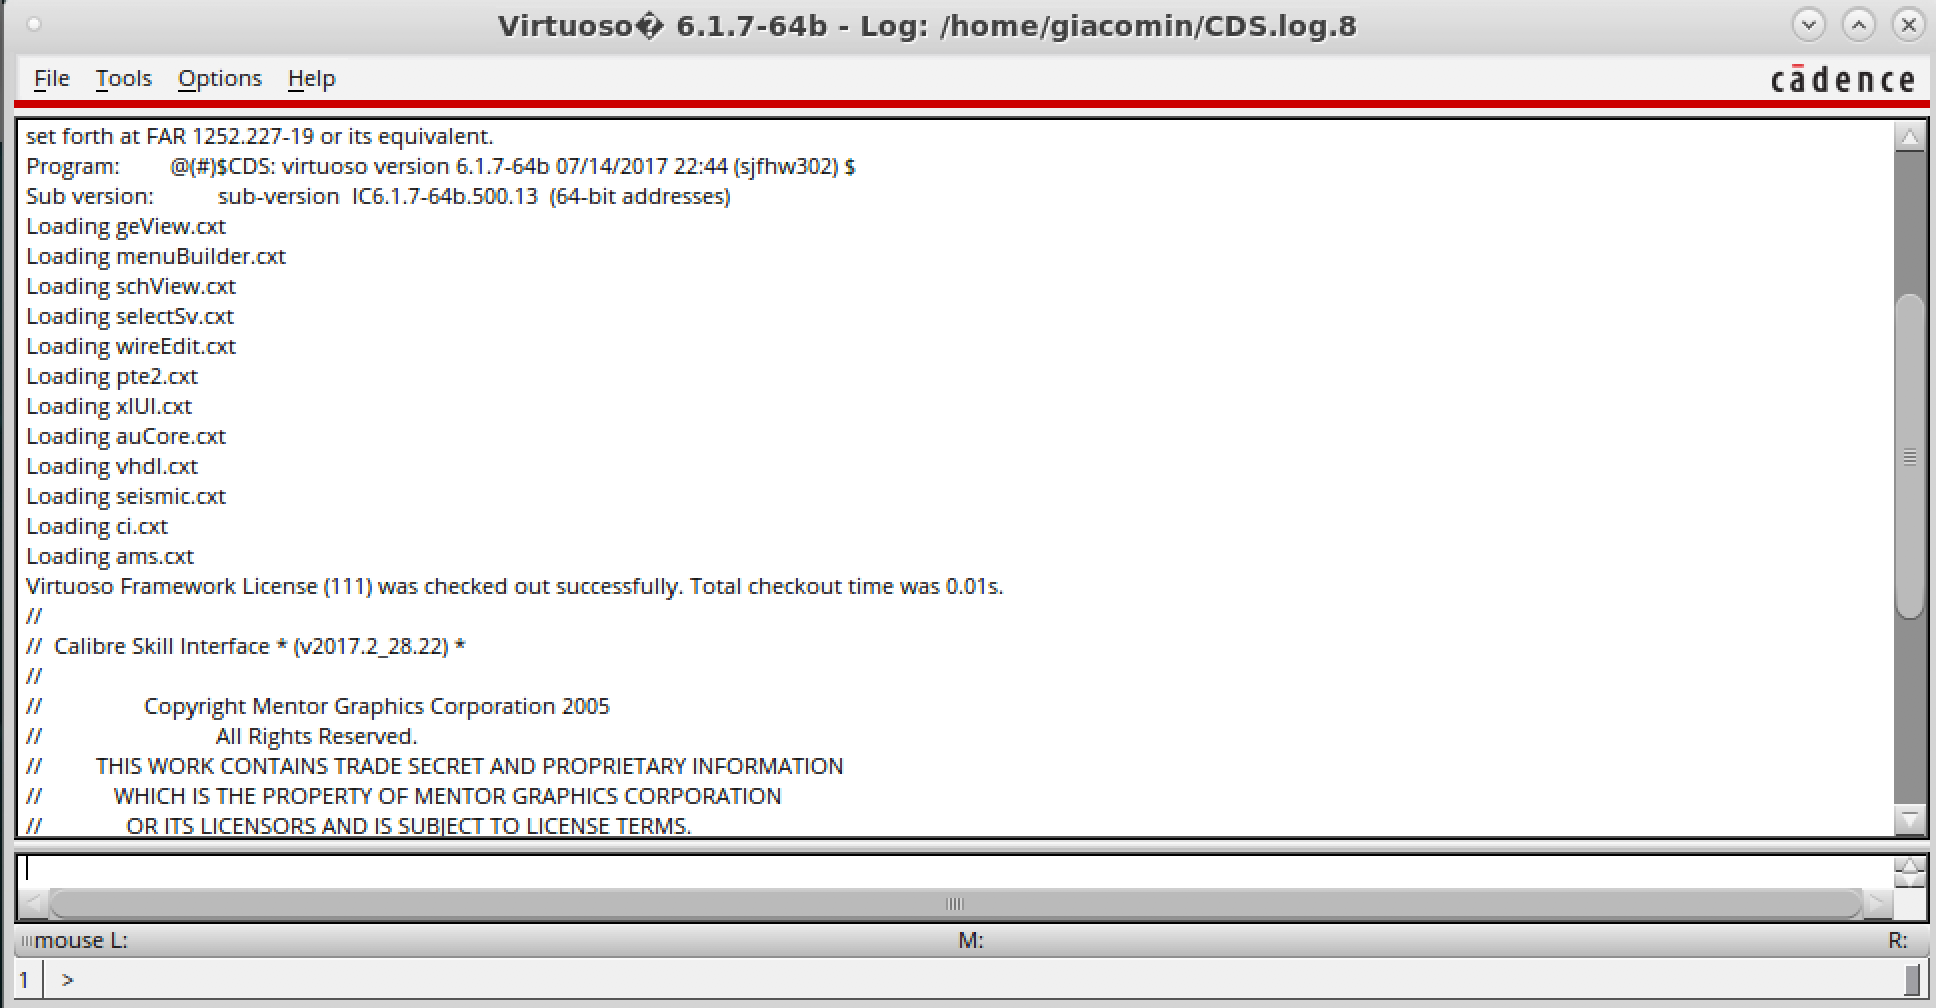
\includegraphics[scale=0.37]{figures/lab1_schematic_sim/ciw}
		\caption{The Command Interpreter Window.}
		\label{fig_ciw}
	\end{figure}
	
	Another window should also pop-up (Fig. \ref{fig_library}): the library manager window. In virtuoso, all the designs are stored in different libraries. Each library contains several cells and each cell is defined through different views (referred as cellviews). A single cell can have multiple cellview that can be different way of representing the cell (schematic, layout, symbol, \textit{etc.}). By default, some libraries are already provided to you: 
	
	\begin{itemize}
		\item \textbf{basic:} contains graphical elements for drawing schematics.
		\item \textbf{analogLib:} contains all the useful elements for electrical simulation (voltage and current sources, ideal resistors and capacitors, switches, ground, \textit{etc.}). This library cells not being physical, this library is only used for simulation purposes.
		\item \textbf{s8phirs$\_$10r:} contains all the core devices (transistors, resistors, capacitors) from the SkyWater 130$nm$ technology node. You will use those devices to create your own designs.
	\end{itemize}	
	\begin{figure}[!h]
		\centering
		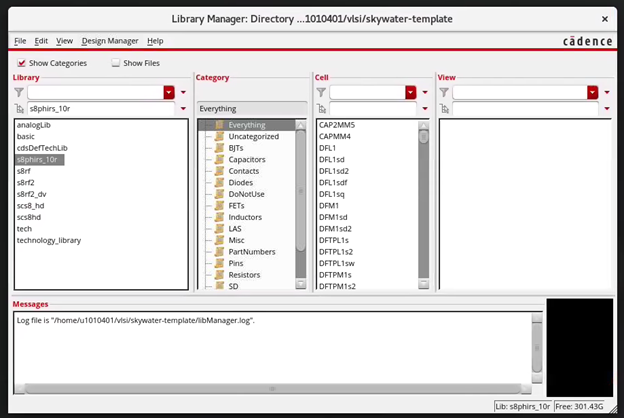
\includegraphics[scale=0.21]{figures/lab1_schematic_sim/library}
		\caption{The Library Manager window.}
		\label{fig_library}
	\end{figure}
	
	\parbox[t]{\dimexpr\textwidth-\leftmargin}{%
		\begin{wrapfigure}[11]{r}{0.5\textwidth}
			\vspace{0mm}
			\centering
			\vspace{-\baselineskip}
			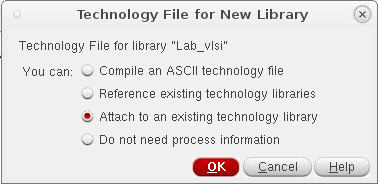
\includegraphics[scale=0.6]{figures/lab1_schematic_sim/lib}
			\caption{Technology file choice for new library.}
			\label{fig_lib}
		\end{wrapfigure}
		\item Now, you first need to create a new library for your designs (referred as your design library). Create a new library in Virtuoso\textsuperscript{\tiny\textregistered} \textit{(Library Manager -> File -> New -> Library…)}. After choosing the location of your library (it is recommended to put it in the \textbf{/libs} directory inside your current working directory to ensure a better organization), a pop-up window appears, as shown in Fig \ref{fig_lib}. 
		\item Select \textit{Attach to an existing technology library} and select \textit{$s8phis$\_$10r$}. By doing this, your design library will use the same technology process (physical layers, layout rules, \textit{etc}.) than the provided Skywater 130\emph{nm} library by the foundry. \newline } 
	
	
	
	
	\item For the rest of this lab and the following labs, when creating new cells, place them in the design library you just created.
\end{enumerate}
\subsection{Technology Characterization}
\subsubsection{Creating the Schematic}
In this section, you will first characterize the technology you are using. It is always a good practice to first draw an I-V curve of the transistors you work with to study their characteristics such as $I_{on}$, $I_{off}$, \textit{etc}.
\begin{remark}
	In this part, you will create a single schematic cellview for your \textit{nmos} transistor and the voltage sources you will use to perform the I-V characterization. However, in the rest of the lab, it is suggested to always create a schematic cellview for your logic gate (i.e. inverter, OR) and another schematic cellview for your testbench (where you instantiate the voltage sources as well as the gate previously defined). In that way, it allows some flexibility since your gate cellview can be reused in multiple testbenches. 
\end{remark}	
\begin{warning}
When defining a new name for a cell or a library, only letters, numbers and underscore ($\_$) should be used. Avoid using special characters, such as $\textemdash$, . * $\textbackslash$ or $\slash$
\end{warning}




\begin{enumerate}


	\parbox[t]{\dimexpr\textwidth-\leftmargin}{%
	\begin{wrapfigure}[22]{r}{0.42\textwidth}
		\vspace{0mm}
		\centering
		\vspace{-\baselineskip}
		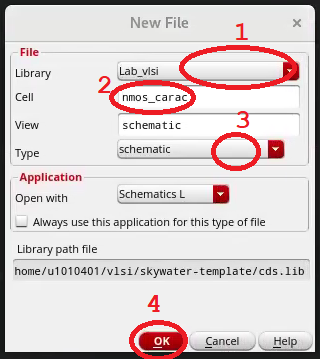
\includegraphics[scale=0.6]{figures/lab1_schematic_sim/newcell.png}
\caption{Creating a new cell.}
\label{fig_newcell}
	\end{wrapfigure}
	\item Create a new cell for the \textit{nmos} characterization (\textit{File -> New -> Cellview...}). Verify that your design library is selected in the \textit{Library} field. Specify the name of your cell in the \textit{name} field (such as \textit{nmos$\_$carac}). For now, you will perform an electrical simulation through a schematic so choose the schematic type, as depicted in Fig. \ref{fig_newcell}, and click OK.
\item 	A cell named nmos$\_$carac is now created, with one view called schematic and the Virtuoso\textsuperscript{\tiny\textregistered} Schematic Editor L window should pop-up, allowing you to edit your new cellview (Fig. \ref{fig_schematicL}). The \textbf{\textcolor{blue}{Navigator}} part allows you to quickly browse through all the devices, pins, nets, \textit{etc.} of your design. The \textbf{\textcolor{blue}{Property editor}} allows you to quickly change the property of the currently selected device. The \textbf{\textcolor{blue}{Schematic display area}} is where you will instantiate all the components, voltage sources, \textit{etc.}} 

	\begin{figure}[!h]
		\centering
		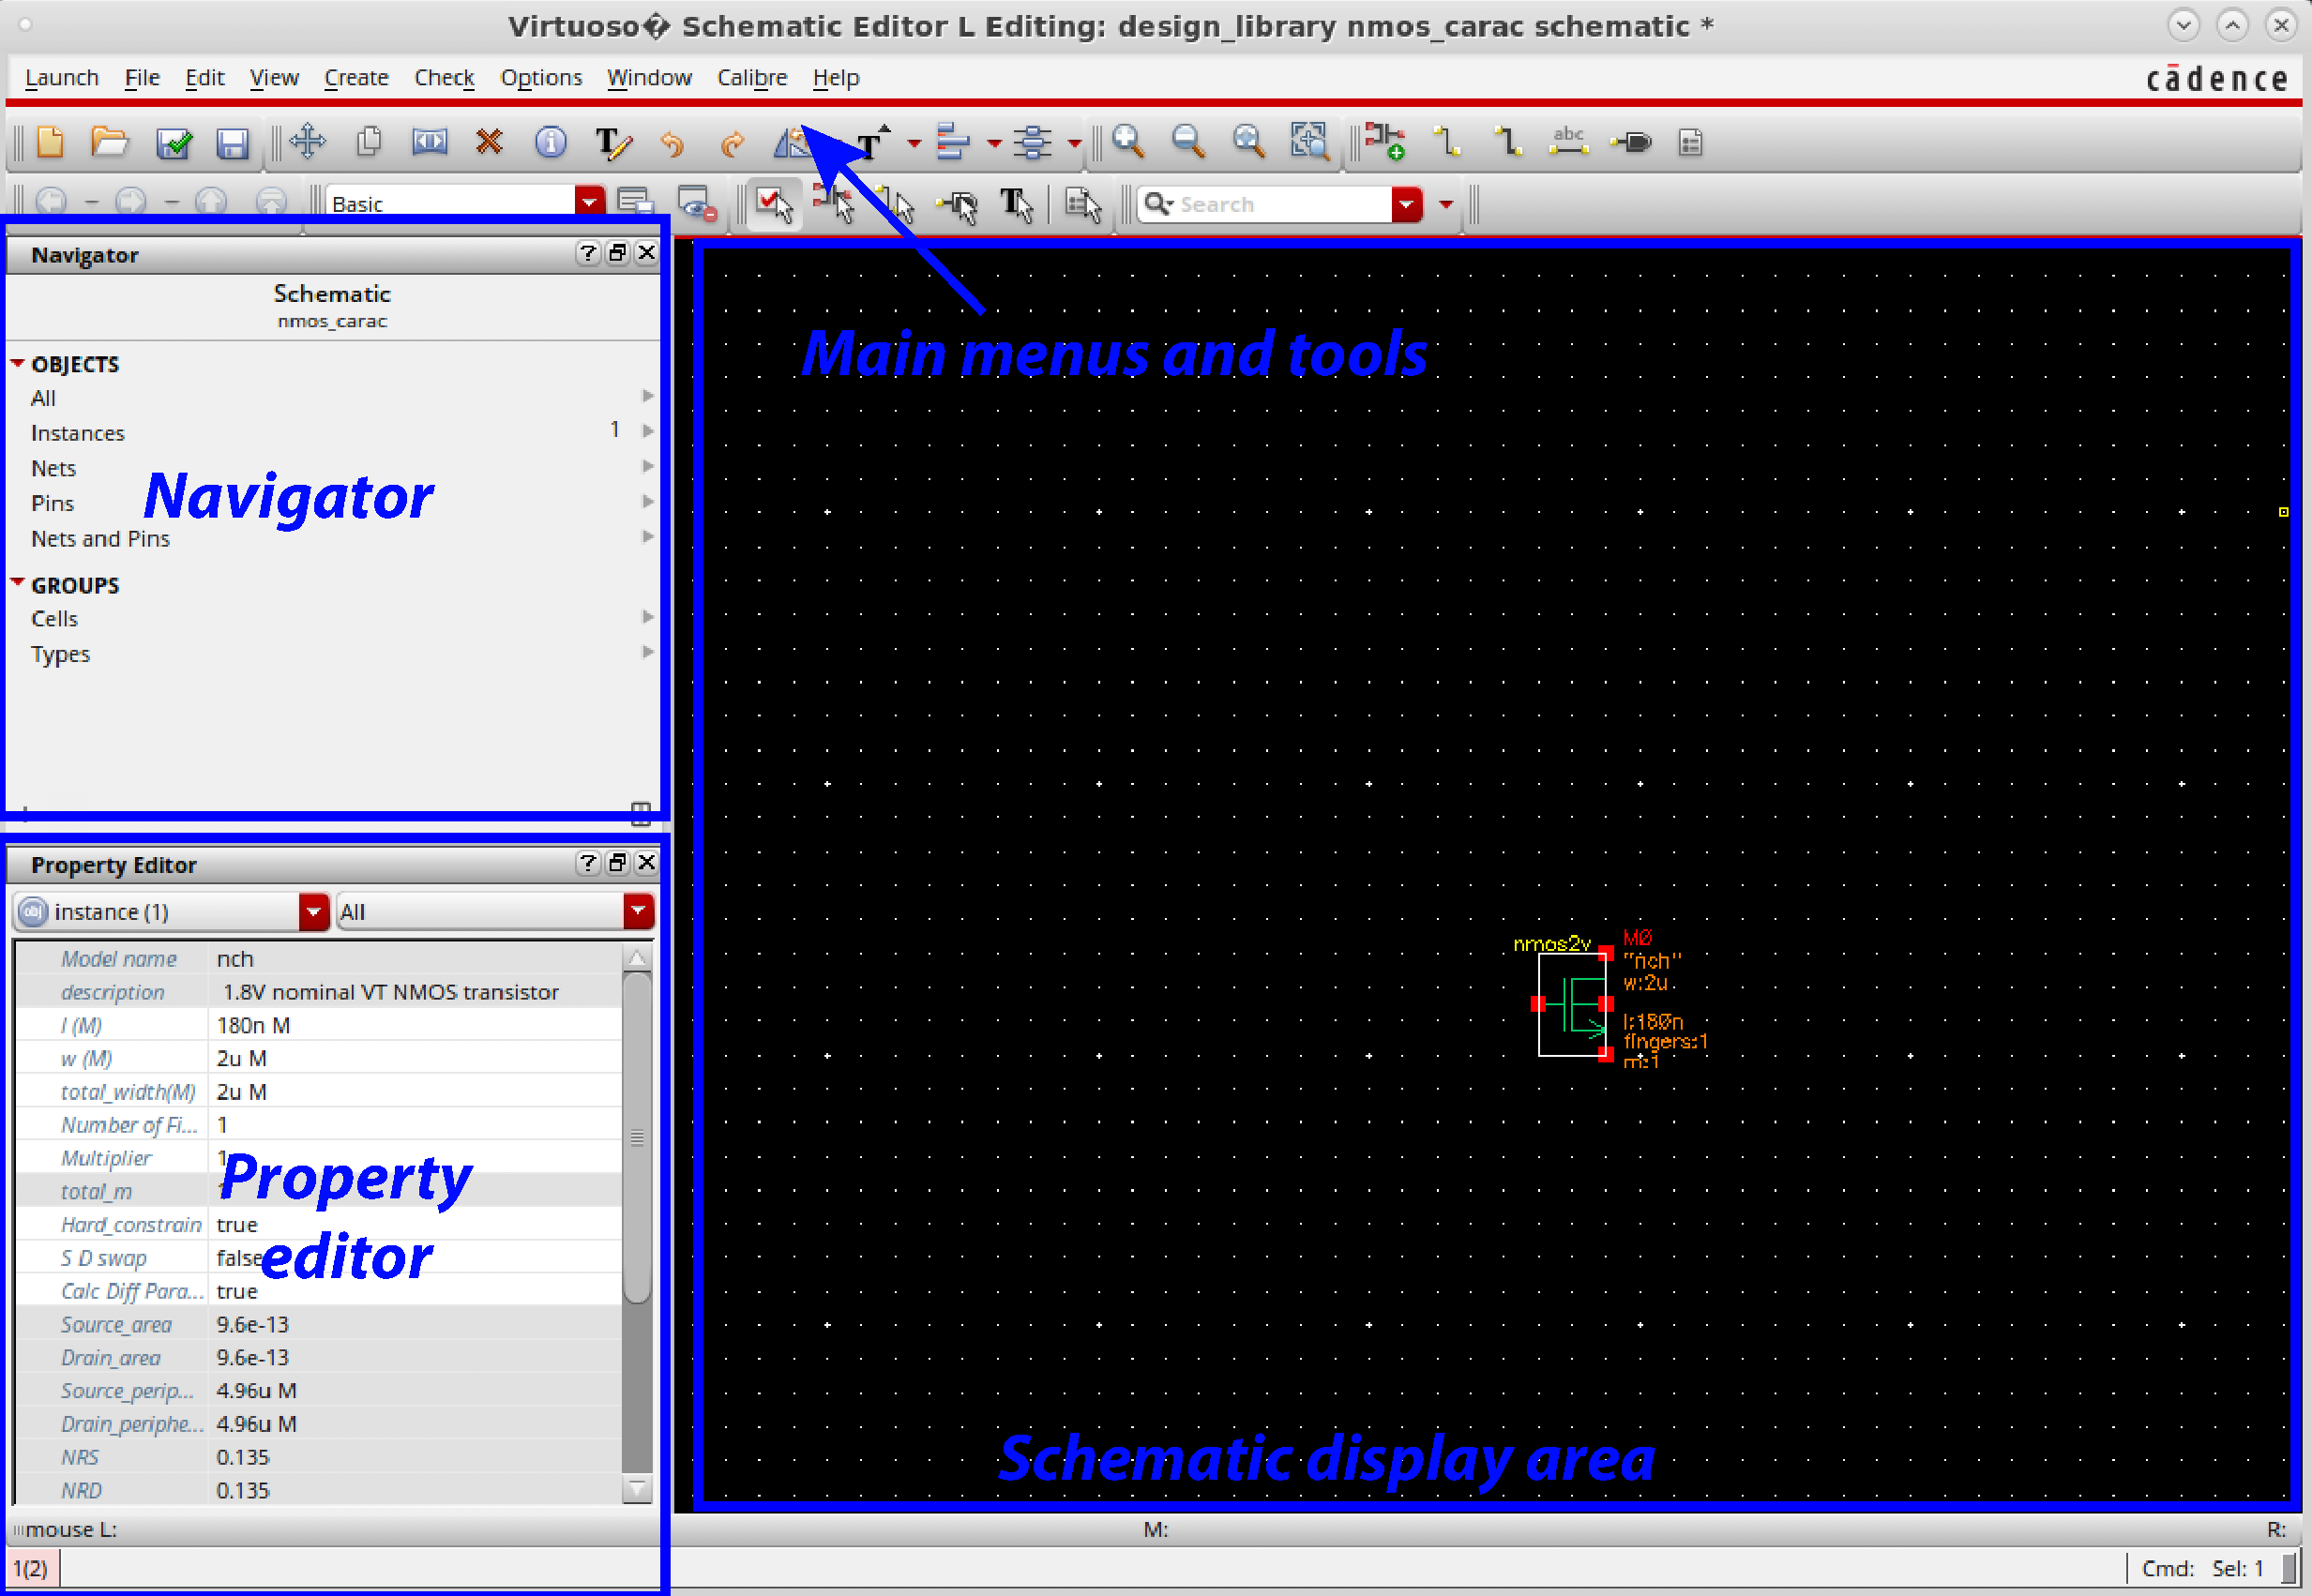
\includegraphics[scale=0.32]{figures/lab1_schematic_sim/schematicL.pdf}
		\caption{Schematic editor L window.}
		\label{fig_schematicL}
	\end{figure}
	
	
	\parbox[t]{\dimexpr\textwidth-\leftmargin}{%
		\begin{wrapfigure}[22]{r}{0.4\textwidth}
			\vspace{-0mm}
			\centering
			\vspace{-\baselineskip}
			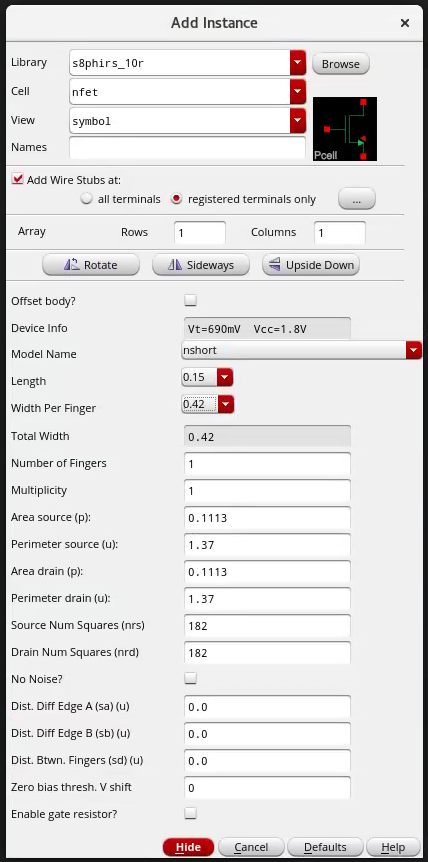
\includegraphics[scale=0.35]{figures/lab1_schematic_sim/instanciate}
			\caption{Component instantiation window.}
			\label{fig_instantiate}
		\end{wrapfigure}
		
		\item First, instantiate (\textit{Create -> Instance...} or press \textbf{i}) an $nmos$ transistor (\textit{$nfet$} from the \textit{$s8phis$\_$10r$} library), as shown in \ref{fig_instantiate}. $nfet$ and $pfet$ are the regular 1.8V $nmos$ and $pmos$ transistors you will use for all your designs in the remaining of the labs.
		\item Try to move your transistor on the display area to get more familiar with the tool. To do so, press \textbf{m}, click one the transistor and move it across the display area. Click again to place it where you want.
		\item Check the transistor width. To do so, click on the transistor and press \textbf{q} (or click on the transistor and modify its width directly through the property editor as explained earlier). From the window, you can modify it width, length, number of fingers, \textit{etc.}. Set the Model Name to nshort, and check that its width is $420nm$ ($.42um$). This is the smallest size given by default with the Skywater PDK. For the rest of the labs, you will generally use this size for transistors (but also take into account the fact that $pmos$ transistors have to be larger than $nmos$ and you also need to size your transistors accordingly when transistors are in series).\newline } 
	
	\parbox[t]{\dimexpr\textwidth-\leftmargin}{%
		\begin{wrapfigure}[7]{r}{0.5\textwidth}
			\vspace{-0mm}
			\centering
			\vspace{-\baselineskip}
			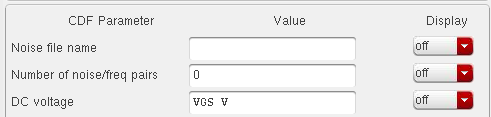
\includegraphics[scale=0.5]{figures/lab1_schematic_sim/paramdc}
			\caption{DC source parameter setup.}
			\label{fig_paramdc}
		\end{wrapfigure}
		\item Instantiate two voltage DC sources (\textit{vdc} from the \textit{analogLib} library) and place them in your design. One will be used to provide the gate voltage and the other one will be used for the drain voltage so place them near those terminals.
		\item Connect the voltage sources correctly to the drain and gate of your transistor. To do so, you need to create some wires to connect the different parts of your circuit ((\textit{Create -> Wire (Narrow)} or press \textbf{w}) and join the two points you want to connect.\newline } 
	
	\begin{remark}
		After pressing \textbf{w} to create a wire, you can press \textbf{s} (snap) so the wire will automatically connect to the closest pin from your mouse.
	\end{remark}
	
	\item Connect the bottom pin of your voltage sources to the ground. You need to use the \textit{gnd} instance from the \textit{analogLib} library.
	\item In the same manner, connect the source of your $nmos$ to the ground. Do not forget to connect the bulk to the ground as well since you are using an $nmos$.
	
	
	
	\parbox[t]{\dimexpr\textwidth-\leftmargin}{%
		\begin{wrapfigure}[12]{r}{0.3\textwidth}
			\vspace{-0mm}
			\centering
			\vspace{-\baselineskip}
			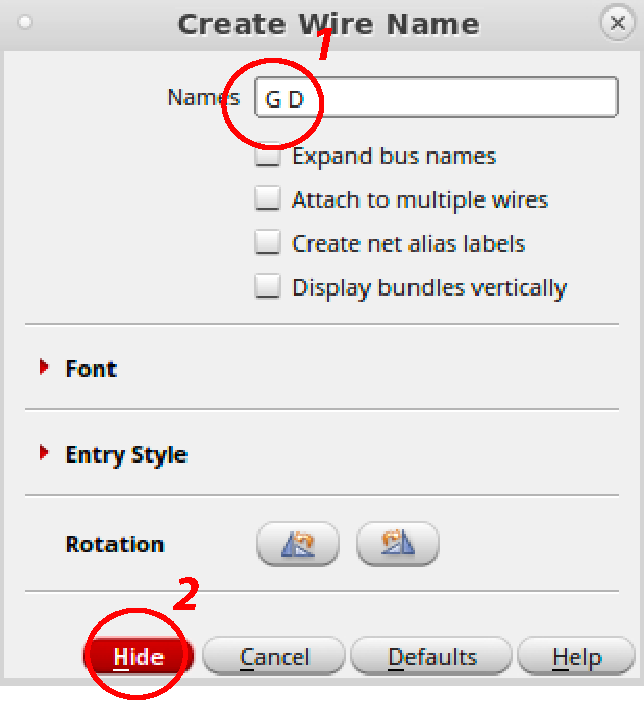
\includegraphics[scale=0.4]{figures/lab1_schematic_sim/label.pdf}
			\caption{Label creation.}
			\label{fig_label}
		\end{wrapfigure}
		\item Edit each of your voltage sources (click on it and press \textbf{q}) to specify the DC voltage as a variable as shown in Fig. \ref{fig_paramdc}. In that way, the voltage of your sources are defined as global variables and you will be able to directly modify them later in your simulation. 
		\item Create some labels for the important wires (in this case, the drain D and gate G of your transistor). All the connected wires are electrically at the same potential and together define a \textbf{net}. It will also help you to know which curve is what when doing the simulation (otherwise the names are assigned randomly). To do so, \textit{Create -> Wire Name...} or press \textbf{l}. Then specify the name(s) of the wire(s) you want to label and click Ok, as depicted in Fig. \ref{fig_label}. Then, click on the respective wire(s) you want to label from your schematic.\newline } 
	
	\parbox[t]{\dimexpr\textwidth-\leftmargin}{%
		\begin{wrapfigure}[12]{r}{0.6\textwidth}
			\vspace{-0mm}
			\centering
			\vspace{-\baselineskip}
			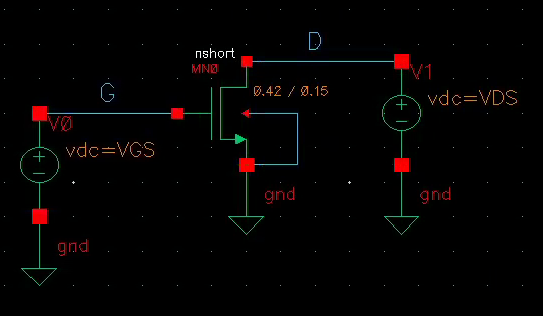
\includegraphics[scale=0.6]{figures/lab1_schematic_sim/nmos_carac}
			\caption{$nmos$ transistor testbench schematic.}
			\label{fig_nmos_carac}
		\end{wrapfigure}
		\item Check and Save your schematic (\textit{File -> Check and Save} or \textbf{Shift + X}). The schematic will be checked for potential errors. If there are any errors or warnings, a dialog box will inform you about them and the CIW will display a detailed message for each problem found.
		\item Your schematic should look like Fig. \ref{fig_nmos_carac}.\newline } 
	
	
\end{enumerate}
\newpage
\subsubsection{Performing the Simulation}
\begin{enumerate}
	\parbox[t]{\dimexpr\textwidth-\leftmargin}{%
		\begin{wrapfigure}[16]{r}{0.6\textwidth}
			\vspace{-0mm}
			\centering
			\vspace{-\baselineskip}
			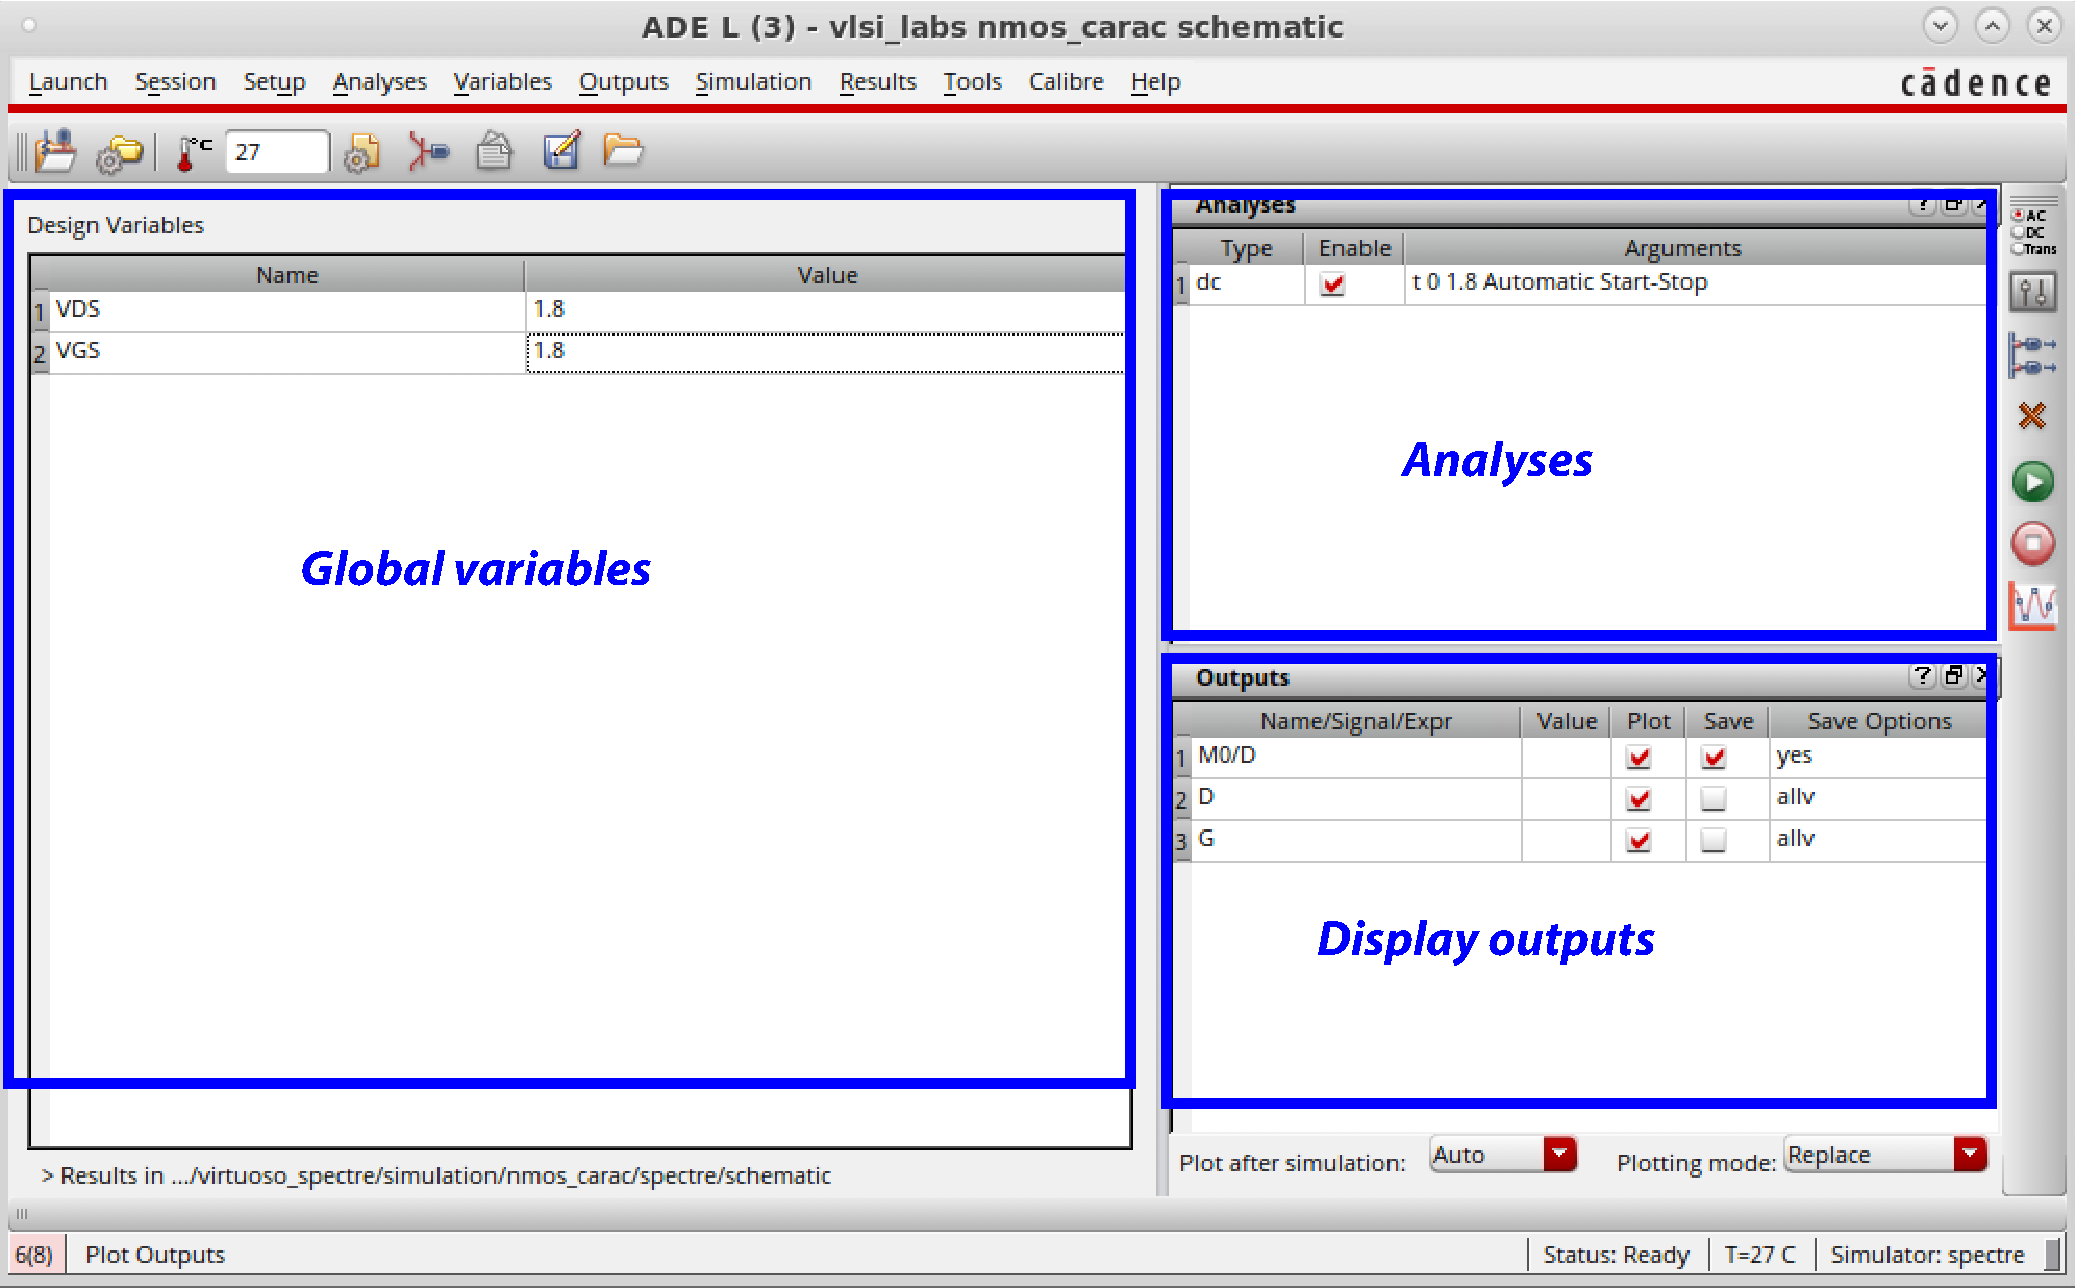
\includegraphics[scale=0.3]{figures/lab1_schematic_sim/ADE.pdf}
			\caption{ADE L window.}
			\label{fig_adel}
		\end{wrapfigure}
		\item Launch the simulation environment (\textit{Launch -> ADE L}). The ADE L window should appear (Fig. \ref{fig_adel}). The \textbf{\textcolor{blue}{Global variables}} is where all your design variables are defined (transistor width or length, source voltages, \textit{etc.}). Note that only the variables you define as a parameter in your schematic can be used as global variable. The \textbf{\textcolor{blue}{Analyses}} panel defines the different analyses you will run on your schematic (transient, DC, AC, \textit{etc.}). The \textbf{\textcolor{blue}{Display outputs}} is where you choose which output (voltage, current, parameter) will be displayed after the simulation.
		\newline } 
	
	
	\parbox[t]{\dimexpr\textwidth-\leftmargin}{%
		\begin{wrapfigure}[22]{r}{0.35\textwidth}
			\vspace{-0mm}
			\centering
			\vspace{-\baselineskip}
			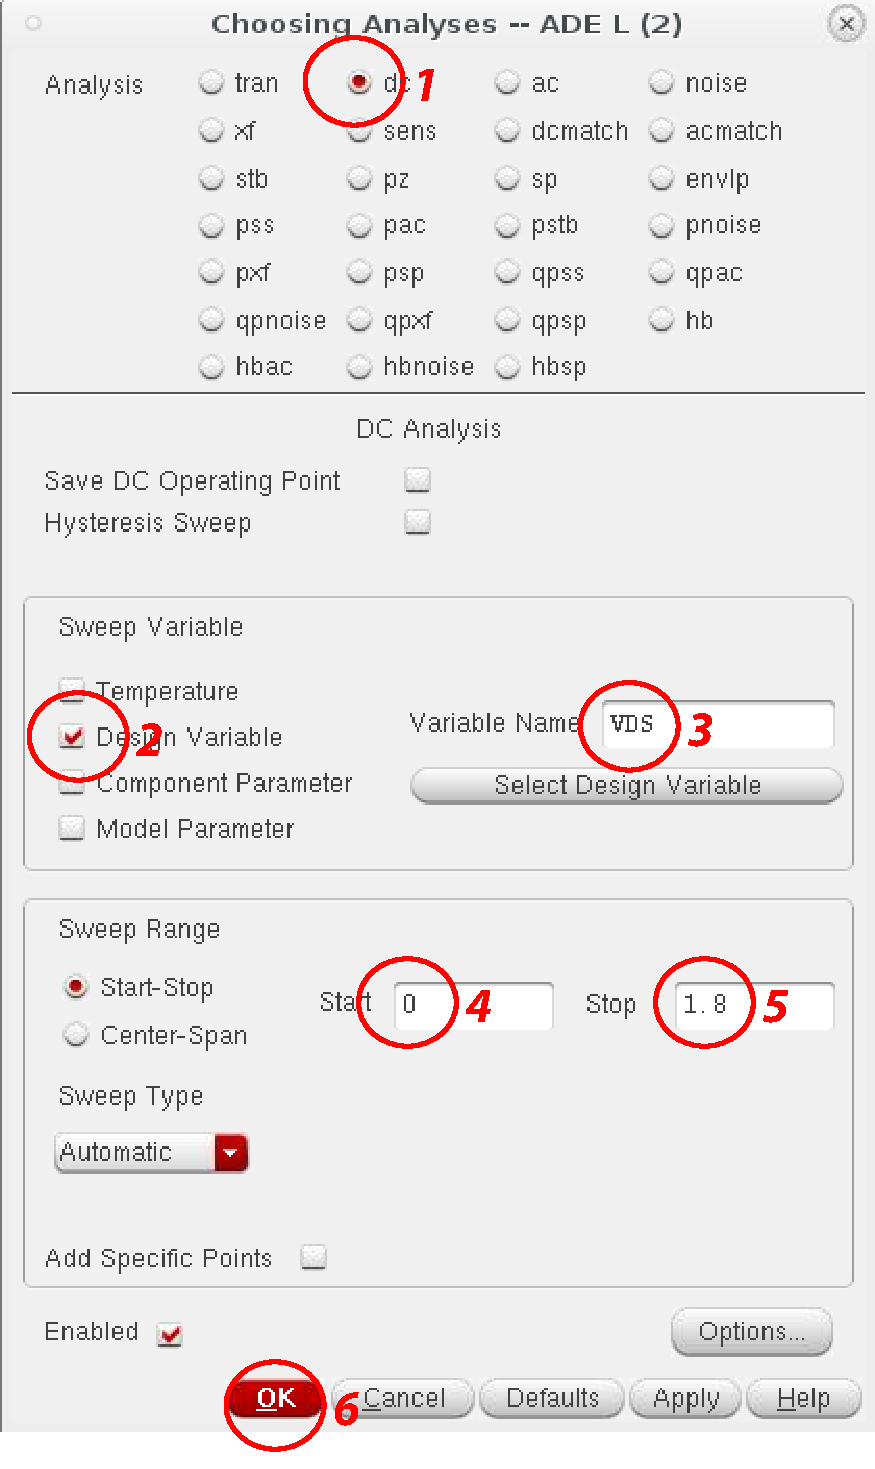
\includegraphics[scale=0.4]{figures/lab1_schematic_sim/dcsweep.pdf}
			\caption{DC sweep analysis.}
			\label{fig_dcsweep}
		\end{wrapfigure}
		\item First, you need to import your design variables (in this case the gate and drain source voltage you previously defined as parameters) to be able to define their value. To do so, go on the ADE window and do: \textit{Variables -> Copy from Cellview}. Don't forget to specify an initial value for your parameter in the left field, otherwise, the simulation will not run. In our case, we can set both voltages to the nominal supply voltage of this technology node: 1.8V.
		\begin{warning}
		In the ADE environment, when specifying a value (after importing your variable for instance, do not indicate their unit).
		\end{warning}
		\item Specify which kind of simulation you want to run. In this case, we are doing a DC simulation (\textit{Analyses -> Choose... -> dc}) and we want to draw an I-V curve so we need to sweep the drain voltage from $0$ to $1.8V$. To do so, you need to select the $design variable$ option, choose the variable name as $VDS$ and sweep if from $0$ to $1.8V$, as illustrated in Fig. \ref{fig_dcsweep}.
		\item Select which outputs you want to plot (\textit{Outputs -> To Be Plotted -> Select On Design}). The schematic window should appear. Select the gate and drain voltage as well as the drain current. Your ADE window should look like the one on Fig. \ref{fig_adel}.
		\begin{remark}
			When selecting which output to display for the ADE, you can select a voltage by clicking on the associated wire. To select a current, click on the associated terminal (red square on the schematic). 
	\end{remark}} 
	\item Run your simulation by clicking on the green triangle button and observe the I-V curve (Fig. \ref{fig_savestate} (a)).
	
	
	
	
	
	\begin{figure}[!h]
		\centering
		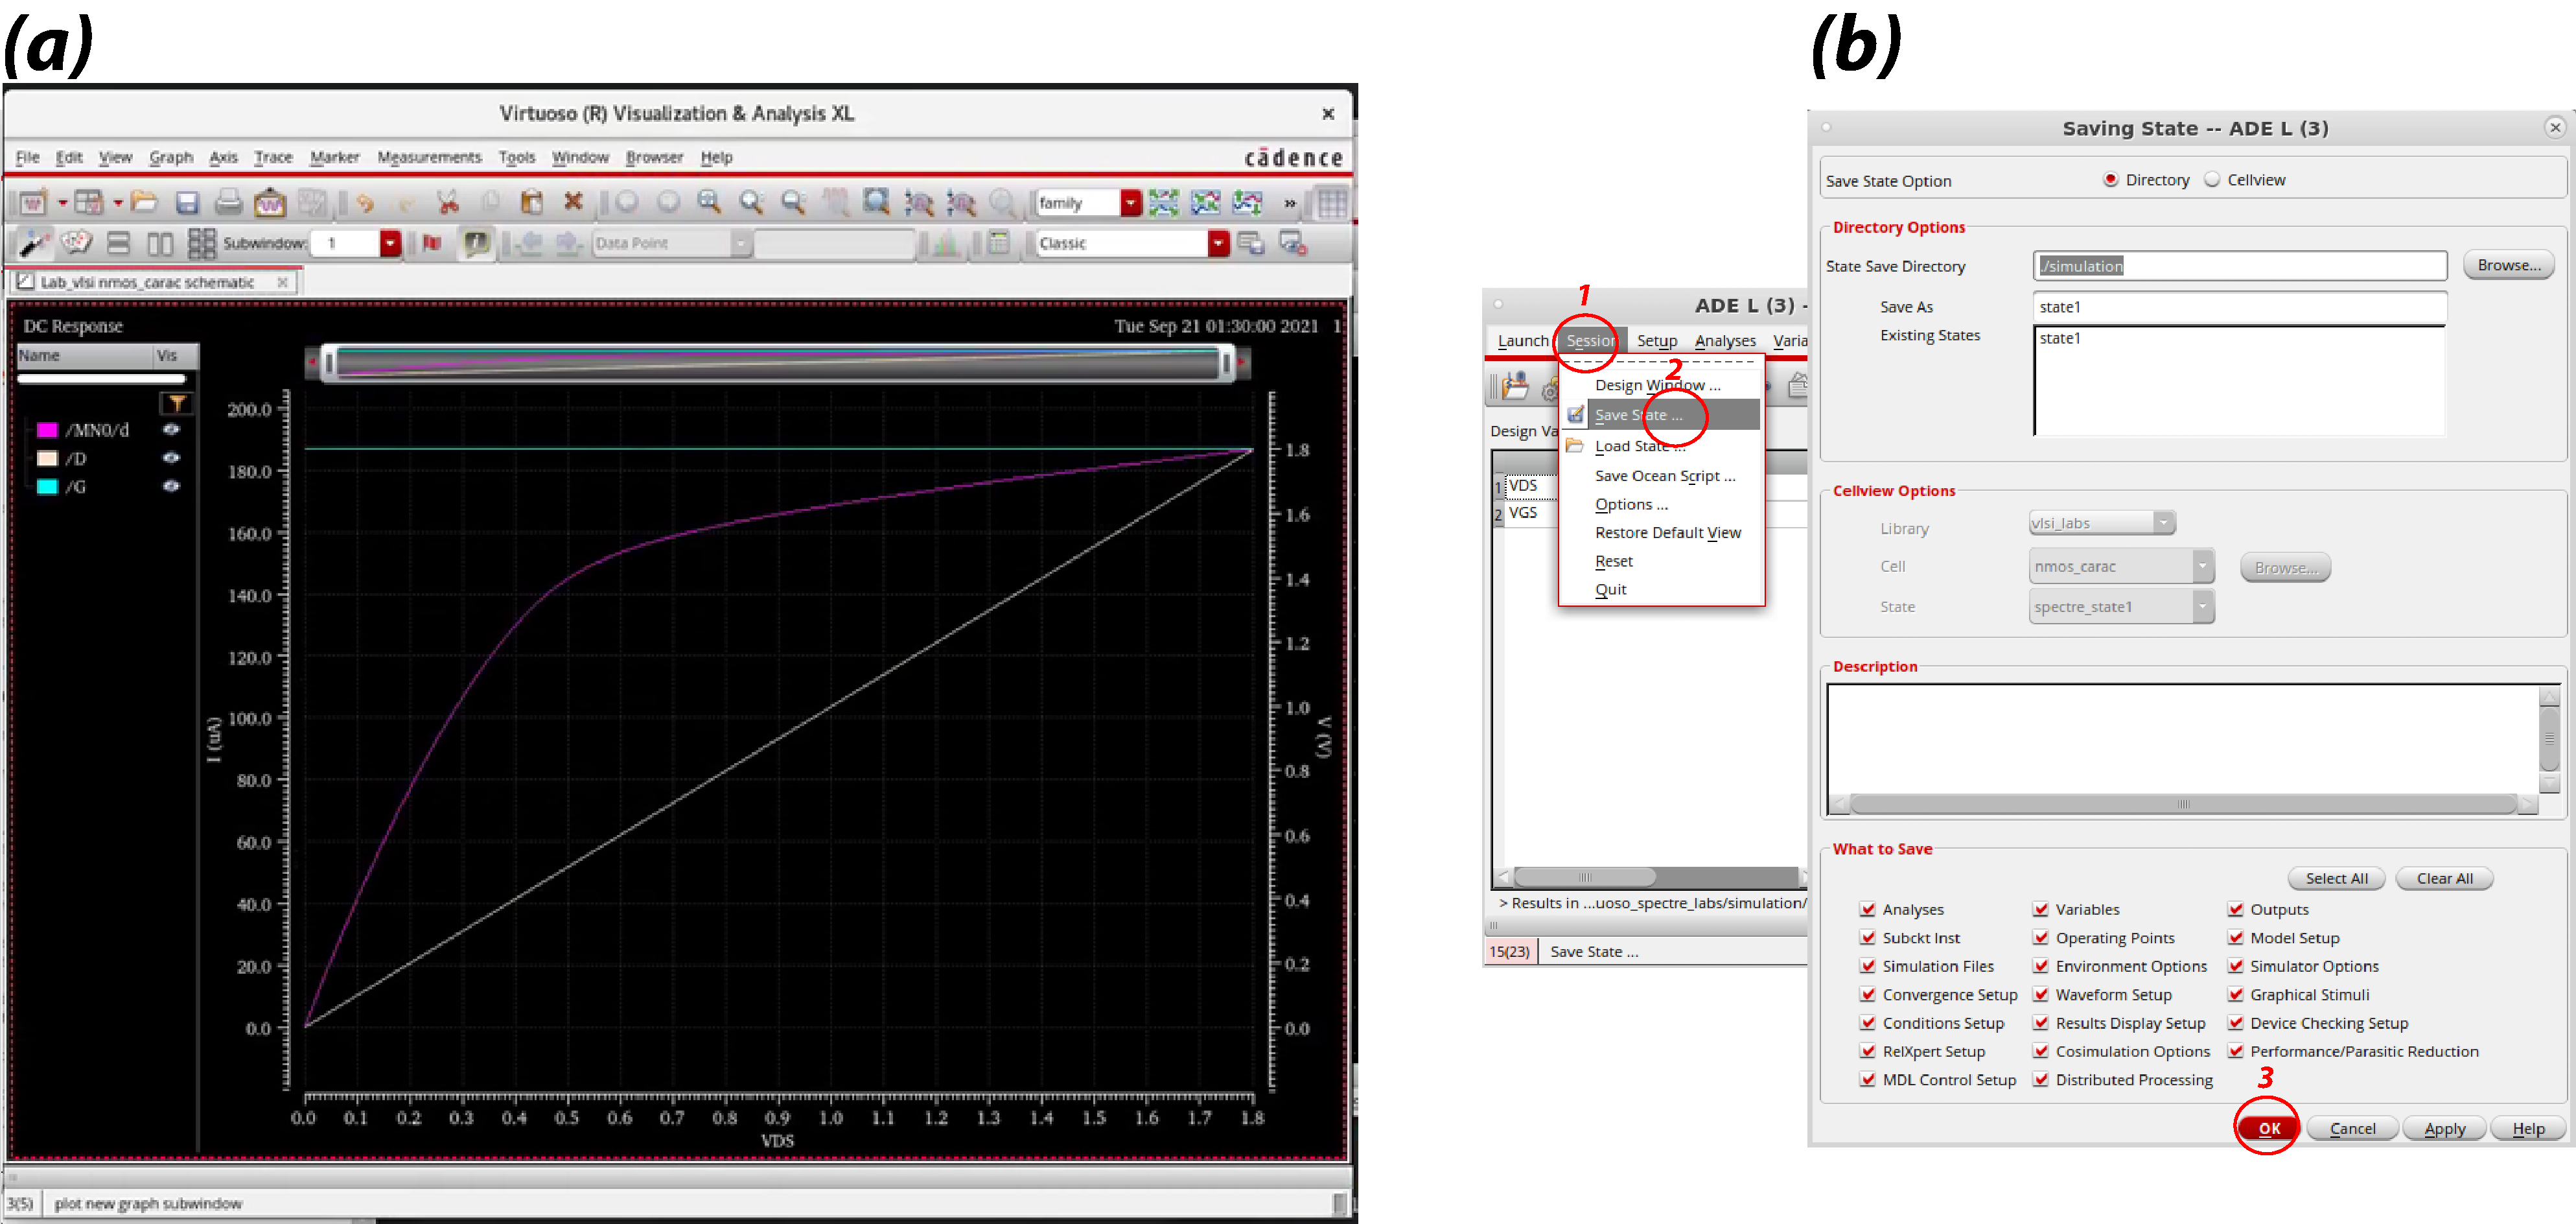
\includegraphics[scale=0.25]{figures/lab1_schematic_sim/save_state}
		\caption{(a) $nmos$ I-V curve; (b) Saving the ADE state.}
		\label{fig_savestate}
	\end{figure}
	
	
	\item Save your ADE L configuration so you can reopen it later without having to re-specify the displayed output signals, the analysis setup, the parameters, \textit{etc}. To do so: \textit{Session -> Save State... -> OK}, as shown in Fig. \ref{fig_savestate} (b).
	
	
	\begin{warning}
		For the rest of the lab, don't forget to save your ADE configuration for each testbench you do. 
	\end{warning}
	
	\item Now, plot the I-V curve for different $VGS$. To do so, you need to run a parametric DC analysis. A parametric analysis allows you to perform several simulations (transient, DC, \textit{etc}.) by sweeping a parameter. In case of a DC simulation, it allows you to sweep another parameter (you will sweep $VDS$ for different $VGS$). To run the parametric analysis, do as follows:
	\begin{enumerate}
		\item From the ADE L window, go to: \textit{Tools -> Parametric Analysis}. You can then choose which parameter to sweep as shown in Fig \ref{fig_paramsweep}. You can also choose the range and the number of steps. Here, you want to sweep $VGS$ from $0$ to $1.8V$ with 10 steps.
		
		\begin{figure}[!h]
			\centering
			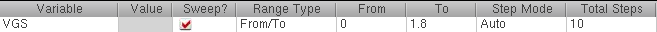
\includegraphics[scale=0.6]{figures/lab1_schematic_sim/paramsweep}
			\caption{Parametric analysis setup for the DC sweep.}
			\label{fig_paramsweep}
		\end{figure}
		
		\item Run your simulation by clicking on the green triangle button from the parametric analysis window and observe the different I-V curves, as depicted in Fig. \ref{fig_paramcurve}.
		
		\begin{figure}[!h]
			\centering
			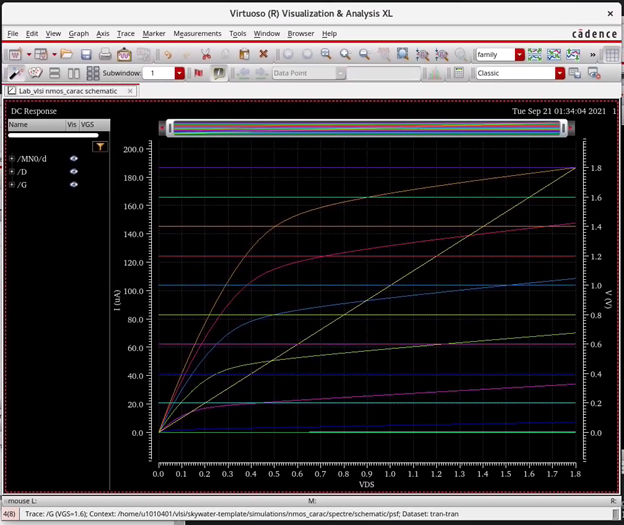
\includegraphics[scale=0.35]{figures/lab1_schematic_sim/parametric_curve}
			\caption{I-V curves for different \textit{VGS}.}
			\label{fig_paramcurve}
		\end{figure}
	\end{enumerate}
	
	
	\begin{exercise}\ \label{ex1}
		\vspace{-5mm}
		\begin{enumerate}
			\item Report the I-V curves under different $VGS$ voltages for your \textit {nmos} transistor.
			\item What are the $I_{on}$, $I_{off}$ of your $nmos$ transistor? Remember that $I_{on}$ is the maximum achievable current and $I_{off}$ if the current when $VDS$ is set to the supply voltage but when the gate is off ($V_{GS}=0V$).
		\end{enumerate}
	\vspace{-5mm}
	\end{exercise}	

\begin{checkpoint}\label{check1}
	Please call an assistant and show him that you obtained the I-V curves for different $VGS$ for your $nmos$ successfully.
\end{checkpoint}	
	
	\item Do the same exercise (create a new cell for it) to characterize a $pmos$ (\textit{$pfet$} from the \textit{$s8phis$\_$10r$} library) transistor. Do not forget that this time, the source of the $pmos$ has to be connected to $V_{DD}$ and that the $pmos$ is $on$ when $V_{GS}=0V$.
	
	\begin{exercise}\label{ex2}
Report the I-V curves under different $VGS$ voltages for your \textit {pmos} transistor as well as its $I_{on}$, $I_{off}$.
	\end{exercise}	
	
	
	\begin{remark}
		Don't forget that the power supply of this technology is $1.8V$. Also, don't forget to perform your I-V characterization for minimum sized $nmos$ and $pmos$ transistors.
	\end{remark}
\end{enumerate}	


\subsection{CMOS Inverter Simulation}
Now, you will create the schematic and symbol of a CMOS inverter. You will also perform some electrical simulations to study its transfer curve as well as its different delays.


\subsubsection{CMOS Inverter Schematic and Symbol Views}	
\begin{enumerate}
	\item Create a new schematic view in your design library for the CMOS inverter (\textit{File -> New -> Cellview...} from the Library Manager) and name it \textit{inv}.
	\item Instantiate two transistors (an $nmos$ and a $pmos$. Use regular transistors (\textit{$nfet$ and $pfet$} from the \textit{$s8phis$\_$10r$} library). The $nmos$ width should be set to $420nm$ (the minimum selectable for the nshort modelname). Set the width of the \textit{pmos} to 2 times the width of the \textit{nmos} (840nm).
	\item Create some wires as previously to connect the two transistors together, following the inverter schematic you saw in class. Don't forget to connect the source and the bulk of the $nmos$ together, as well as for the $pmos$.
	
	
	
	\parbox[t]{\dimexpr\textwidth-\leftmargin}{%
		\begin{wrapfigure}[30]{r}{0.4\textwidth}
			\vspace{-0mm}
			\centering
			\vspace{-\baselineskip}
			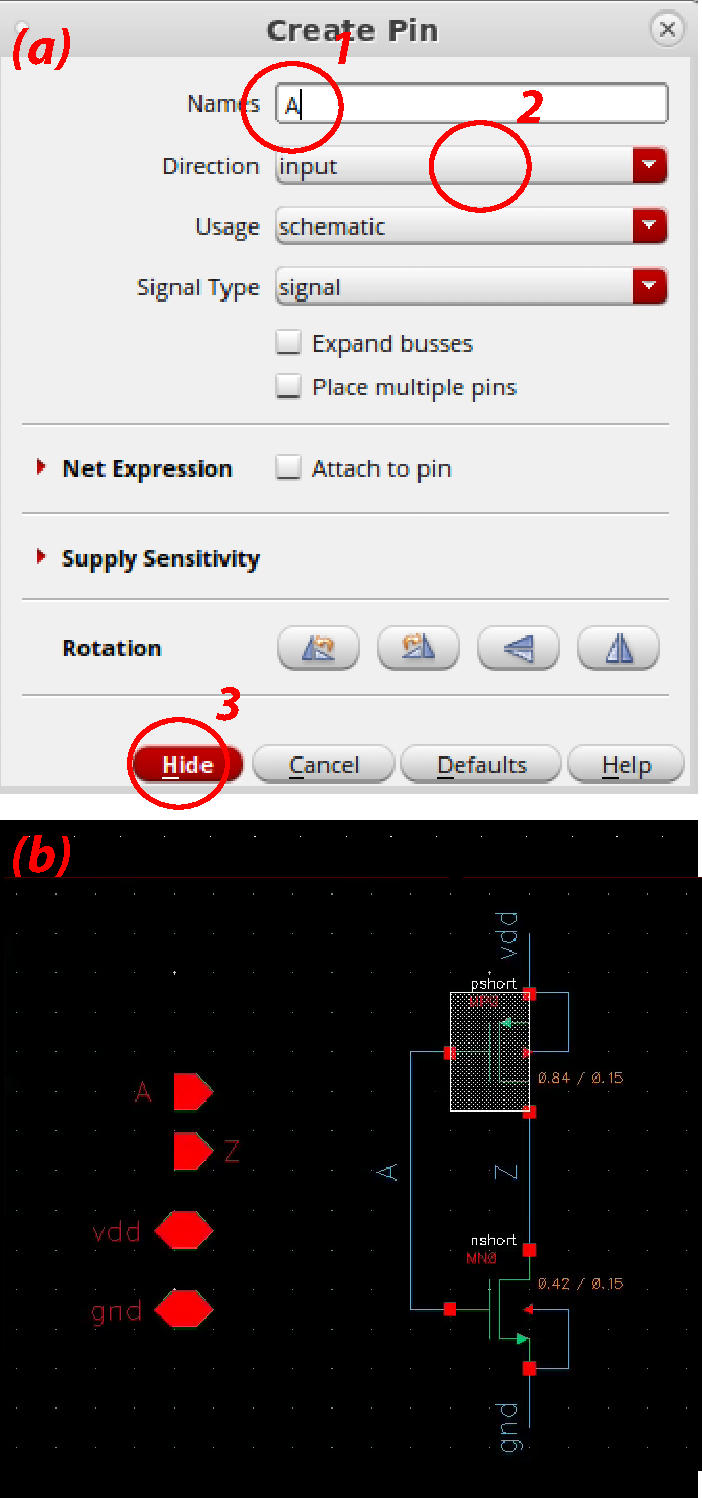
\includegraphics[scale=0.45]{figures/lab1_schematic_sim/pin_schematic.pdf}
			\caption{(a) Schematic pin creation; (b) CMOS inverter schematic.}
			\label{fig_pin}
		\end{wrapfigure}
		\item Create pins for your cell. Pins will define the different connections (interface) between a cell and its environment. If you instantiate a cell in other designs, the only accessible nets will be the previously defined pins. Pins are defined by the name and the direction (input, output or input-output). The purpose of the direction is to check for possible wrong connections (e.g. two outputs shorted together, or floating inputs). Typically, input-output pins are used for power supplies and bidirectional interfaces.
		
		\begin{itemize}
			\item Create the input pin. To do so: \textit{Create -> Pin} or press \textbf{p}. A window appears (Fig. \ref{fig_pin} (a), prompting you to enter the name ($A$) and the direction ($input$) of the pin. Click on \textit{Hide} and place the pin on the schematic. You can either place them directly on the net they are supposed to connect to, or on the left of your schematic (and connect the nets later through some labels).	
			\item Repeat the same process for the output (generally denoted \textit{Z}) and power supply pins ($V_{DD}$ and $G_{ND}$). Don't forget to specify the appropriate direction for each pin.
			\item Your schematic should look like Fig. \ref{fig_pin} (b). Don't forget to Check and Save your schematic and ensure there is no errors or warnings.
	\end{itemize}}
	
	
	\parbox[t]{\dimexpr\textwidth-\leftmargin}{%
		\begin{wrapfigure}[12]{r}{0.5\textwidth}
			\vspace{-0mm}
			\centering
			\vspace{-\baselineskip}
			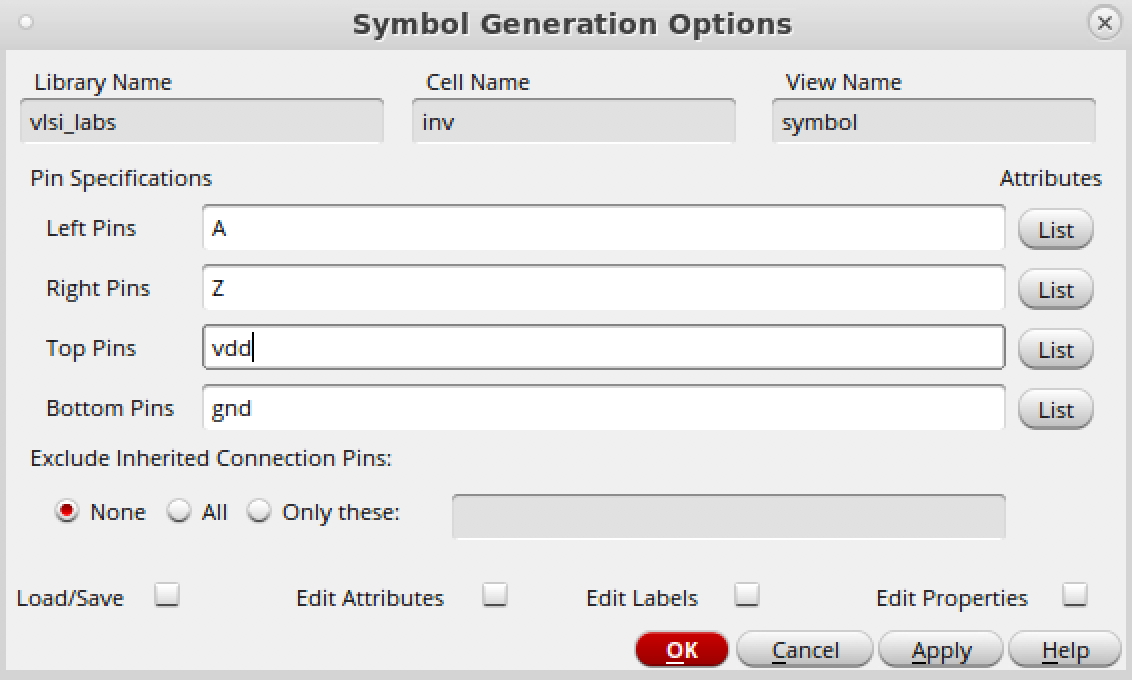
\includegraphics[scale=0.4]{figures/lab1_schematic_sim/cellview}
			\caption{Cellview pin location.}
			\label{fig_cellview}
		\end{wrapfigure}
		\item Check and Save your schematic (\textit{File -> Check and Save} or \textbf{Shift + x}). Verify that there is no errors or warnings.
		\item Now, you will create a symbol for your inverter. A symbol is useful when you work with larger designs and you need to instantiate previously designed gates (e.g. designing an adder with some XOR and AND gates, \textit{etc.}), instead of redrawing the transistor schematic every time. The symbol will provide information on how to connect the cell from the outside. Note that the pins of your symbol should be the same ones defined in your schematic. To do so: 
		\begin{itemize}
			\item On the schematic window, (\textit{Create -> Cellview -> From Cellview..}). 
	\end{itemize} } 
	\begin{itemize}
		\item A window appears. All the options should be set correctly so just press OK.
		\item Another window appears (Fig. \ref{fig_cellview}) where you can specify the location of the pins on your symbol. It is a good practice to set the inputs on the left, the output on the right and the power supply pins on top or bottom, depending on the direction you chose when you defined your schematic pins, the pins should be correctly placed here.		
		\item Click OK.
		\item Shape your symbol how you want it, as depicted in Fig. \ref{fig_invsymbol} and Check and Save it. There should be no warnings or errors. 
		\begin{remark}
			You don’t need to change the $[$@instanceName$]$ and $[$@partName$]$ labels in the generated symbol. When you instantiate the cell, these labels will display the instance name and the cell name respectively. By default, the instances you place in a schematic will be named I0, I1, I2, \textit{etc}. To change the name of an instance, select the instance and press $Q$.
			
		\end{remark}
		
		\begin{figure}[!h]
			\centering
			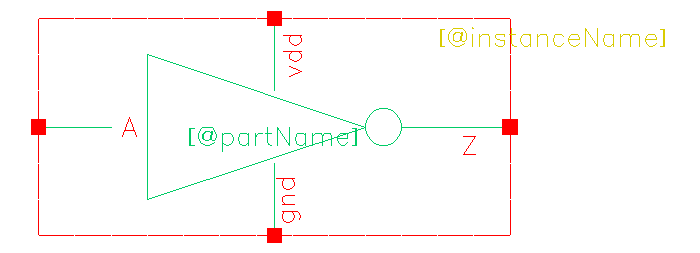
\includegraphics[scale=0.45]{figures/lab1_schematic_sim/inv_symbol}
			\caption{Inverter symbol.}
			\label{fig_invsymbol}
		\end{figure}
	\end{itemize} 
	
\end{enumerate} 
\clearpage
\subsubsection{CMOS Inverter Testbench View}	
You previously created a schematic view of your inverter. However, this view only contains transistors. To perform electrical simulations on it, you need to create a view where you will instantiate some voltage sources, ground points, \textit{etc}. To do so, you need to create a new schematic cellview for your testbench in which you will instantiate your inverter.
\begin{enumerate}
	\item Go to the Library Manager and create a new schematic cellview ($inv\_testbench\_dc$ for instance). 
	\item Instantiate your inverter (you need to select the appropriate library and the inverter symbol cellview you just created) in your schematic.
	\item We will study the \textit{Voltage Transfer Characteristic} of the inverter so you first need to connect the input of your inverter to a DC source voltage ($vdc$ from the $analogLib$). Edit its property to specify the DC voltage as a parameter $VIN$.
	\item Instantiate another DC voltage source for the power supply. Set its DC voltage as a global parameter (VDD). 
	\item For the $V_{DD}$ and $G_{ND}$ symbols, use the $vdd$ and $gnd$ cells from the $analogLib$ library.
	\item For the load capacitor, use the $cap$ cell from the $analogLib$ library and sets its capacitance value to $10f F$.
	\item Don't forget to label your nets (input and output).
	\item Your testbench should look like Fig. \ref{fig_invtb}.
	
	\begin{figure}[!h]
		\centering
		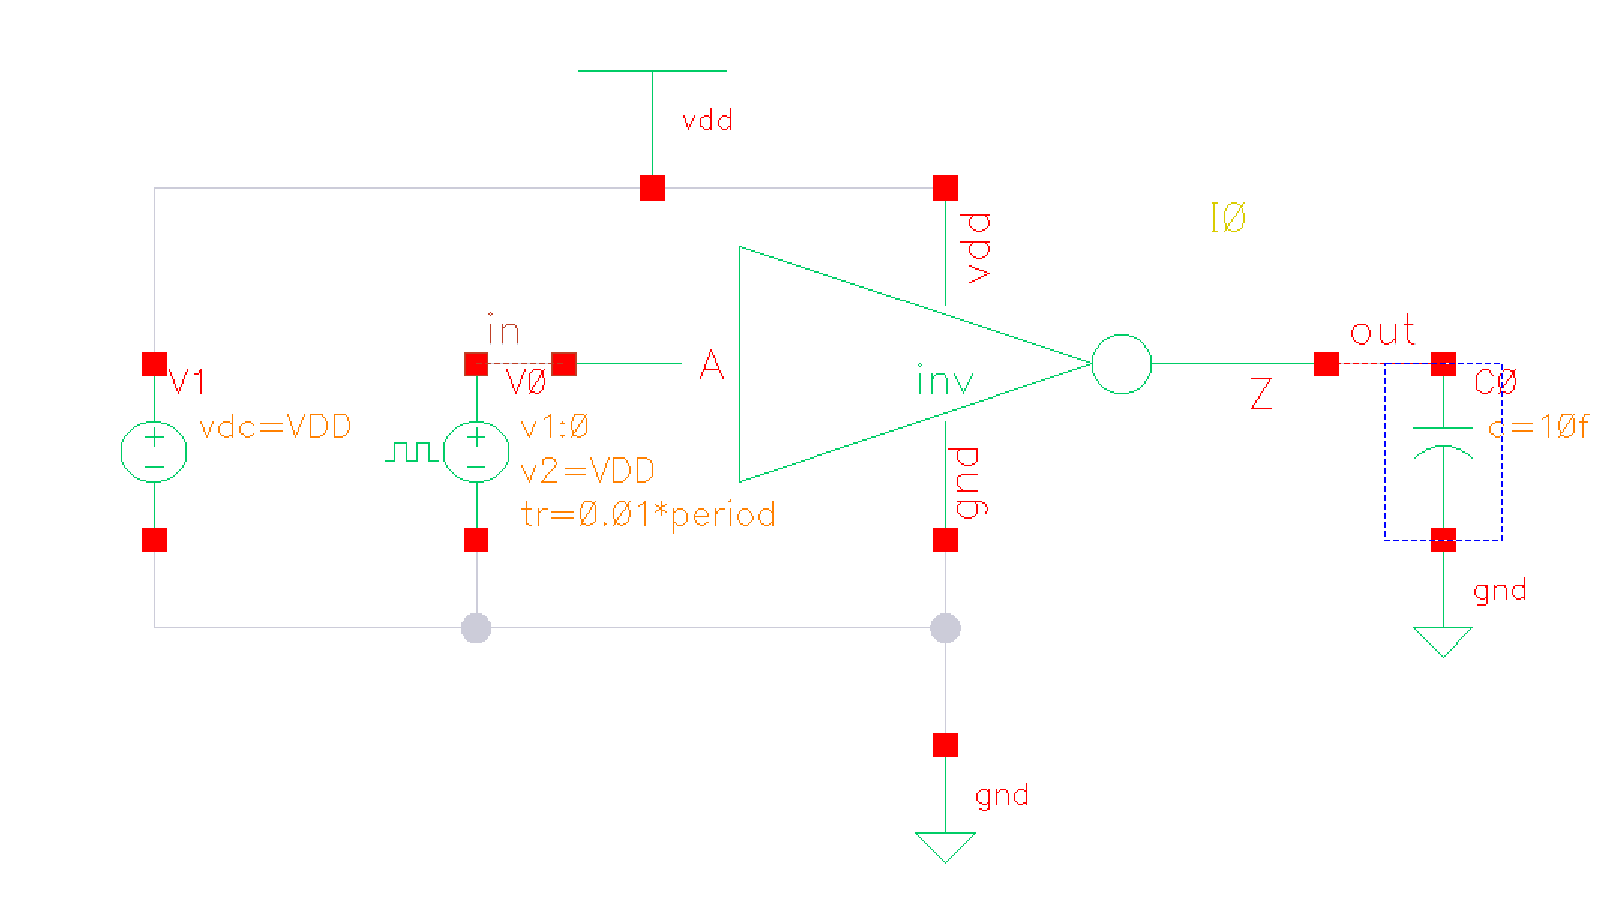
\includegraphics[scale=0.45]{figures/lab1_schematic_sim/inv_tb.pdf}
		\caption{Inverter testbench schematic.}
		\label{fig_invtb}
	\end{figure}
\end{enumerate} 
\begin{remark}
	At this point, you should have 2 cells: one for the inverter and one for the inverter testbench (in which the inverter is instantiated). For the rest of the labs, always create a different cell for your testbench and instantiate the standard cell you want to simulate in it.
\end{remark}
\subsubsection{CMOS Inverter DC Simulation}	
In this section, you will perform a DC simulation of an inverter in order to study the effect of the $pmos$ width on the VTC of your inverter.

\begin{enumerate} 
	\item Launch ADE L.
	\item Import your designs variables ($VIN$ and $VDD$) and set them to an initial value of 1.8V.
	\item Select the kind of analysis you want to run. In this case, you want to perform a DC sweep on $VIN$ going from 0V to 1.8V (the setup is really close to what you do previously for the $nmos$ characteristic).
	\item Select the signals to be displayed ($in$ and $out$ here).
	\item Run the simulation. Your curve should look like Fig. \ref{fig_vtc}.
	\begin{figure}[!h]
		\centering
		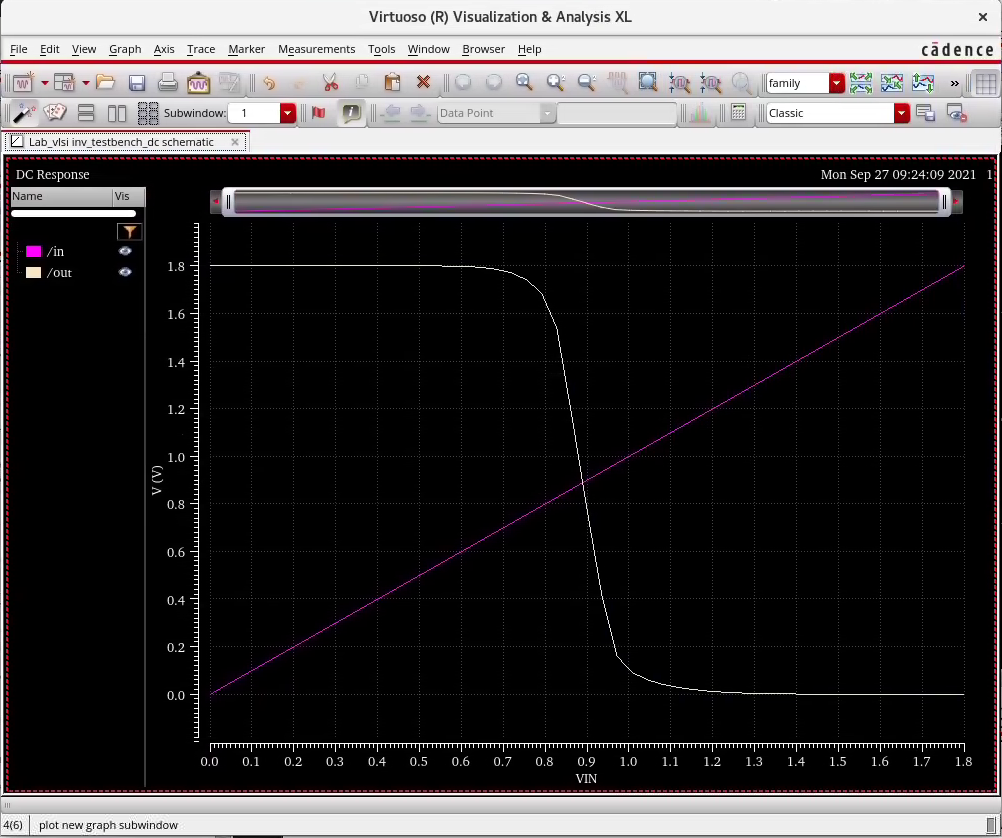
\includegraphics[scale=0.35]{figures/lab1_schematic_sim/vtc_curve}
		\caption{Inverter VTC curve.}
		\label{fig_vtc}
	\end{figure}
	
	\begin{exercise} \label{ex3}
		Plot the Voltage Transfer Curve (VTC), report the switching point of the inverter and specify the dimensions of your transistors.
	\end{exercise}	
	
	
	
	\parbox[t]{\dimexpr\textwidth-\leftmargin}{%
		\begin{wrapfigure}[9]{r}{0.5\textwidth}
			\vspace{-0mm}
			\centering
			\vspace{-\baselineskip}
			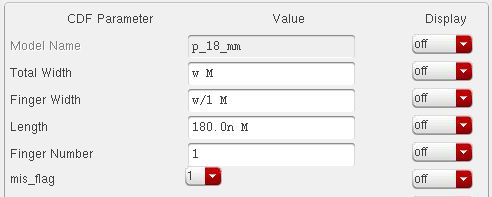
\includegraphics[scale=0.45]{figures/lab1_schematic_sim/width}
			\caption{Setting the transistor width as a parameter.}
			\label{fig_width}
		\end{wrapfigure}
		\item Run a parametric DC analysis for different width of the \textit{pmos} by sweeping the voltage from $0$V to $V_{DD}$. To do so:
		\begin{itemize} 
			\item Go to your inverter cell. To do so, you can either go to the library manager and open the inverter cell directly, or you can directly double click on the inverter symbol from your testbench schematic and click OK (in this case, you went down into the hierarchy. If you want to go back, press \textbf{ctrl + e}).\end{itemize} }
	\begin{itemize} 
		\item Change the width of the \textit{pmos} as a parameter and not a fixed number as shown in Fig \ref{fig_width}.
		\item On the ADE window, do: \textit{Variables -> Copy from Cellview} to import the new width variable on ADE. Don't forget to specify an initial value for your parameter in the left field (840nm for instance).
		\item Go to: \textit{Tools -> Parametric Analysis}. Specify the parameter to sweep as shown in Fig \ref{fig_param} (here \textit w is the width of the \textit{pmos}). 
		\item Run the simulation. \end{itemize} 
	
	
	
	\begin{figure}[!h]
		\centering
		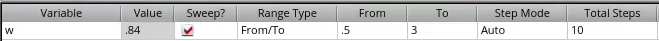
\includegraphics[scale=0.55]{figures/lab1_schematic_sim/param}
		\caption{Parametric analysis setup.}
		\label{fig_param}
	\end{figure}
	
	
	\begin{exercise} \label{ex4}
		Plot the VTC curve for different width of the \textit{pmos}. What is this effect called? Report for which value of the \textit{pmos} width the switching point is equal to $V_{DD}/2$.
	\end{exercise}
	\item As you can see, the \textit{pmos} needs to be very big to have a switching point equals to $V_{DD}/2$. This leads to an unacceptable area and induces big parasitic capacitances. \textbf{For the rest of the labs, we will use the approximation $W_{pmos}=2*W_{nmos}$.}
	
	\begin{remark}
		In the next labs, don't forget to use the same approximation to size your transistors.
	\end{remark}
	\begin{warning}
		Don't forget to change the width value of the \textit{pmos} back to a fixed value (840nm). Otherwise, it will not be able to instantiate the transistor when creating a layout and to pass the LVS since the width will not be fixed.
	\end{warning}

\begin{checkpoint}\label{check2}
	Please call an assistant and show him that you obtained the VTC curve for your inverter successfully.
\end{checkpoint}	


\end{enumerate}

\subsubsection{CMOS Inverter Transient Simulation}	
In this part, we will perform another kind of simulation: transient simulation. It allows to study the behavior of your circuit overt time, when applying a specific input voltage sequence. Since the testbench will be slightly different, a good practice is to create a new testbench view for this particular simulation.
\begin{enumerate}
	
	\parbox[t]{\dimexpr\textwidth-\leftmargin}{%
		\begin{wrapfigure}[18]{r}{0.6\textwidth}
			\vspace{-0mm}
			\centering
			\vspace{-\baselineskip}
			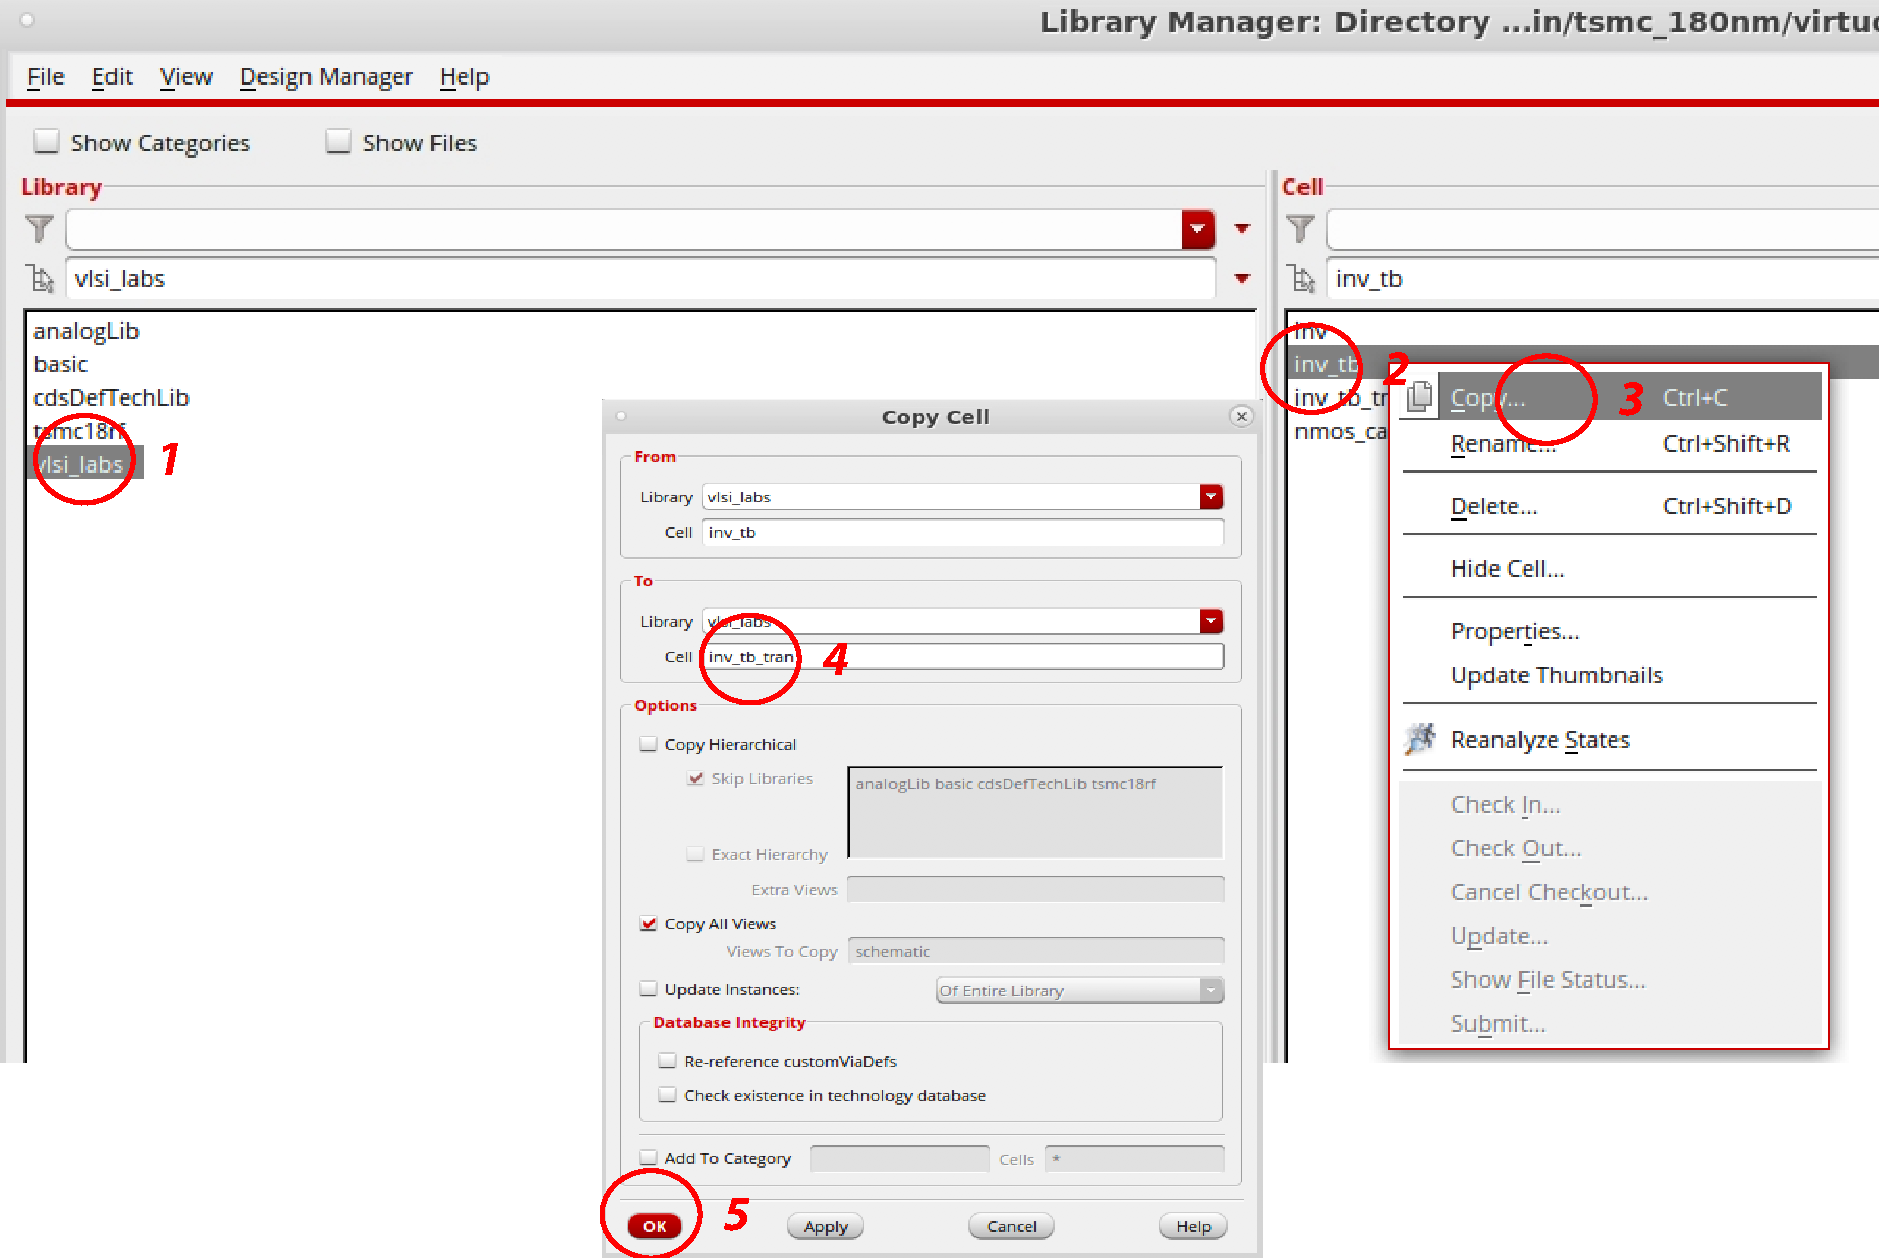
\includegraphics[scale=0.35]{figures/lab1_schematic_sim/copy.pdf}
			\caption{Copying a cell.}
			\label{fig_copy}
		\end{wrapfigure}
		\item First, create a new testbench for the transient simulation. Since the testbench is really similar to the DC simulation (only the input voltage source will change), an easy way to do is to copy the DC testbench and modify it. To do so:
		\begin{itemize}
			\item Go to the Library Manager, select your design library and your inverter testbench cell and right click and on and select $Copy...$.
			\item On the window, select the name you want ($inv\_testbench\_tran$ for instance) for this new testbench in the appropriate field and click OK (Fig. \ref{fig_copy}).
		\end{itemize}
	}
	\begin{itemize}
	\parbox[t]{\dimexpr\textwidth-\leftmargin}{%
	\begin{wrapfigure}[18]{r}{0.6\textwidth}
		\vspace{-0mm}
		\centering
		\vspace{-\baselineskip}
			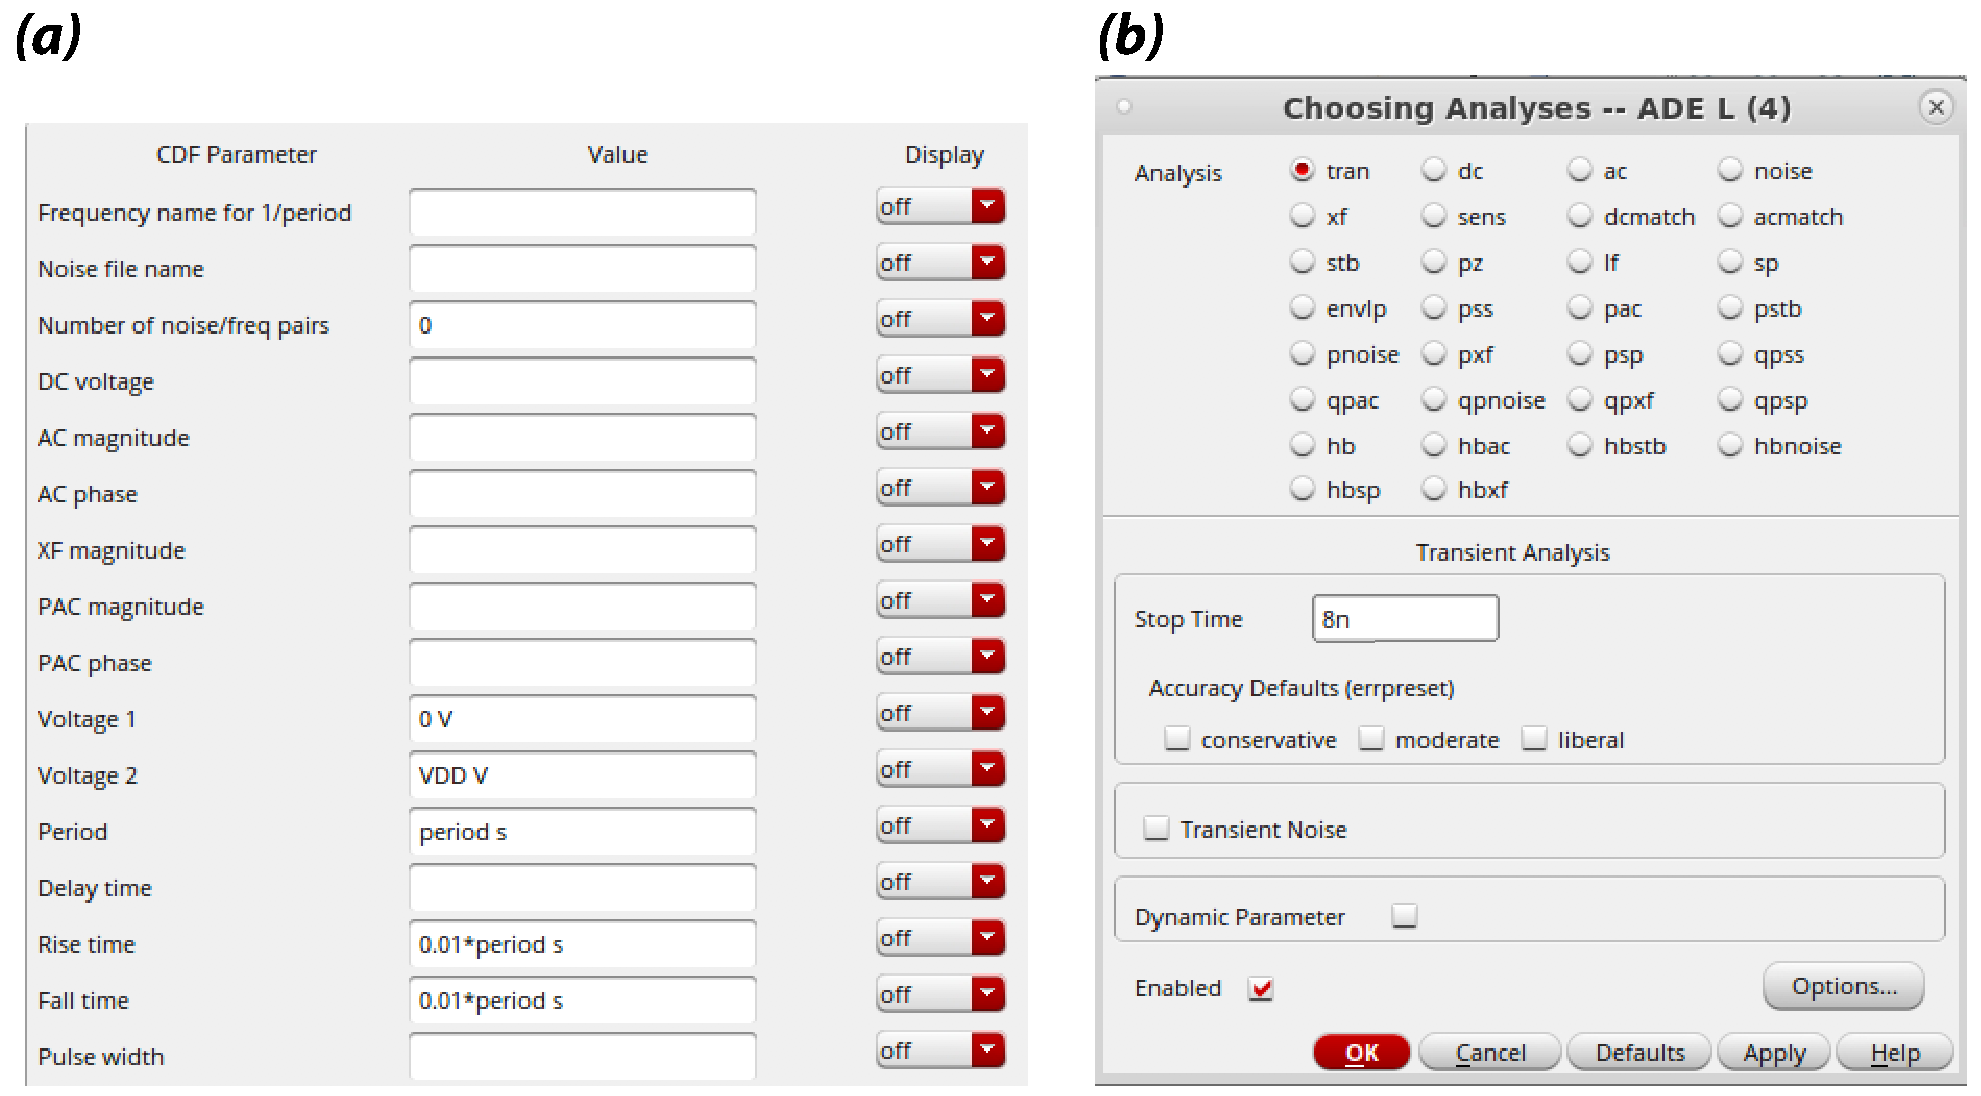
\includegraphics[scale=0.3]{figures/lab1_schematic_sim/tran_pulse}
\caption{(a) Transient simulation parameters; (b) Voltage pulse source parameters.}
\label{fig_pulse}
	\end{wrapfigure}
	\item Open the schematic cellview of your newly created testbench ($inv\_testbench\_dc$) and replace the input (not the supply one) source DC voltage by a pulse source $vpulse$ from the $analogLib$ library.
	\item Specify the parameters of your pulse source as shown in Fig. \ref{fig_pulse} (a). Note that this time, the DC voltage is specify as $Voltage 2$ and not as DC Voltage. Here, the period of your source is specified as a parameter $period$. You will be able to change this parameter in the ADE window later on. The rising and falling times depends on your period.
}
	\end{itemize}

	
	
	\parbox[t]{\dimexpr\textwidth-\leftmargin}{%
		\begin{wrapfigure}[22]{r}{0.5\textwidth}
			\vspace{-0mm}
			\centering
			\vspace{-\baselineskip}
			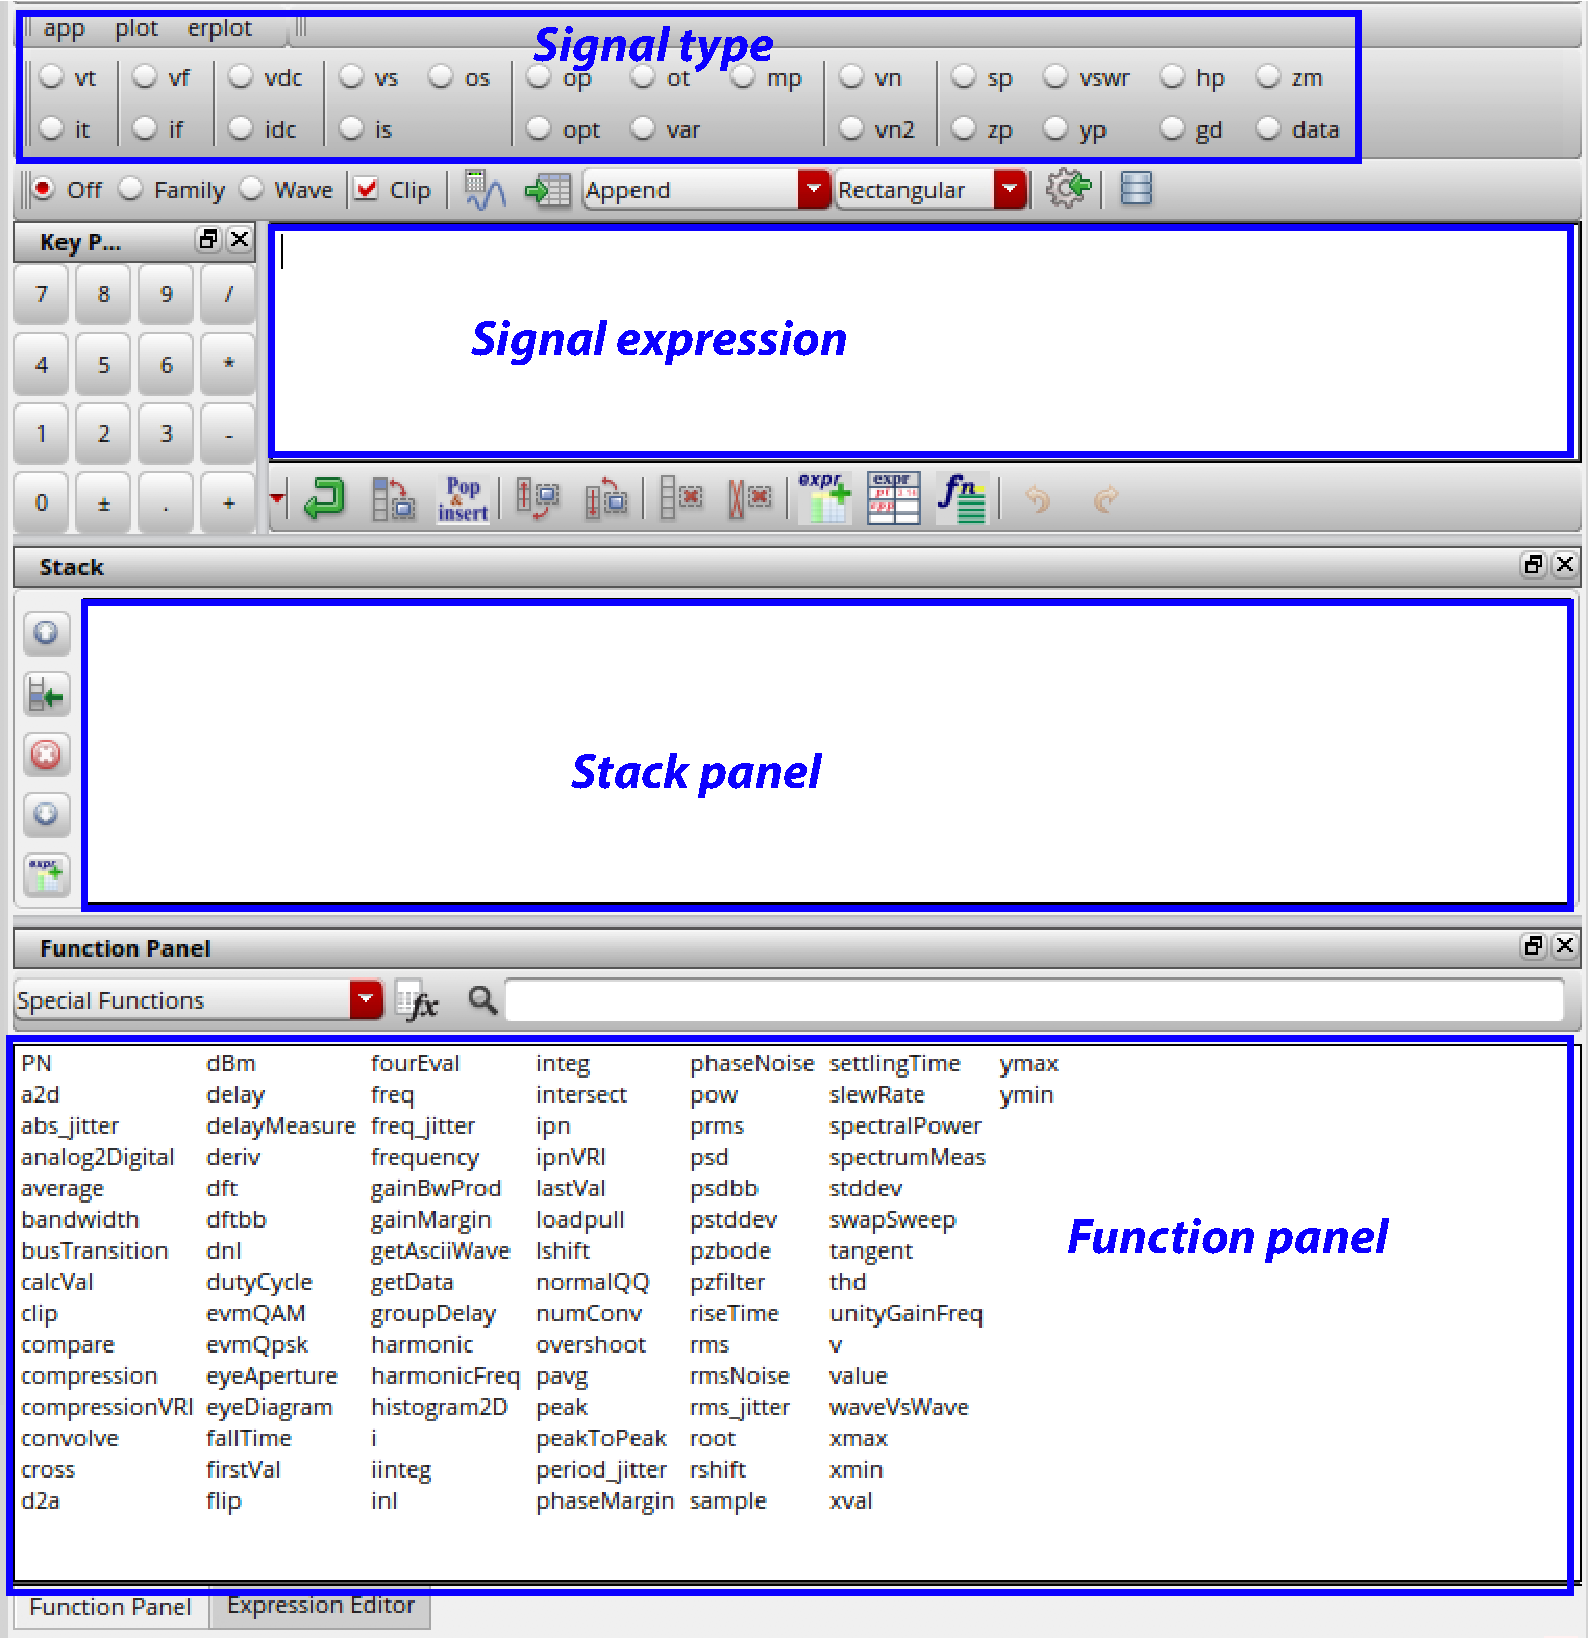
\includegraphics[scale=0.32]{figures/lab1_schematic_sim/calculator_tuto}
			\caption{ADE calculator setup.}
			\label{calculator}
		\end{wrapfigure}
		\item Launch ADE.
		\item Import your design variables and set some initial values. Use a period of 2ns.
		\item Specify a transient analysis (\textit{Analyses -> Choose... -> tran}) as shown in Fig. \ref{fig_pulse} (b) and just specify the stop time (8ns in this case in order to observe 4 period). 
		
		\item Define the delay measurements. To measure some stuff from the curves (falling time, propagation delay, maximum voltage etc.), we will use the Cadence calculator. To do so, first open the Calculator (in the ADE window: \textit{Tools -> Calculator...}).The calculator window should appear, as shown in Fig. \ref{calculator}. The Calculator is a very powerful tool which can help you define expressions and waveforms, plot circuit time or frequency responses, perform useful transforms, signal post-processing and/or analysis. It has many pre-defined mathematical and processing functions and also allows you to define your own functions. \newline
		The \textbf{\textcolor{blue}{Signal type}} panel allows you to choose which type of signal you want to consider (for instance, $vt$ stands for transient voltage). The \textbf{\textcolor{blue}{Signal expression}} panel which displays the expression of the signal you selected from your schematic through the \textbf{\textcolor{blue}{Signal type}} panel. Finally, the \textbf{\textcolor{blue}{Function panel}} allows you to choose which type of function you want to use (delay calculation, frequency response, \textit{etc}). 
	}
	
	\clearpage
	
	
			\item To compute the propagation delay:
	\begin{itemize}
		\parbox[t]{\dimexpr\textwidth-\leftmargin}{%
			\begin{wrapfigure}[21]{r}{0.6\textwidth}
				\vspace{-0mm}
				\centering
				\vspace{-\baselineskip}
				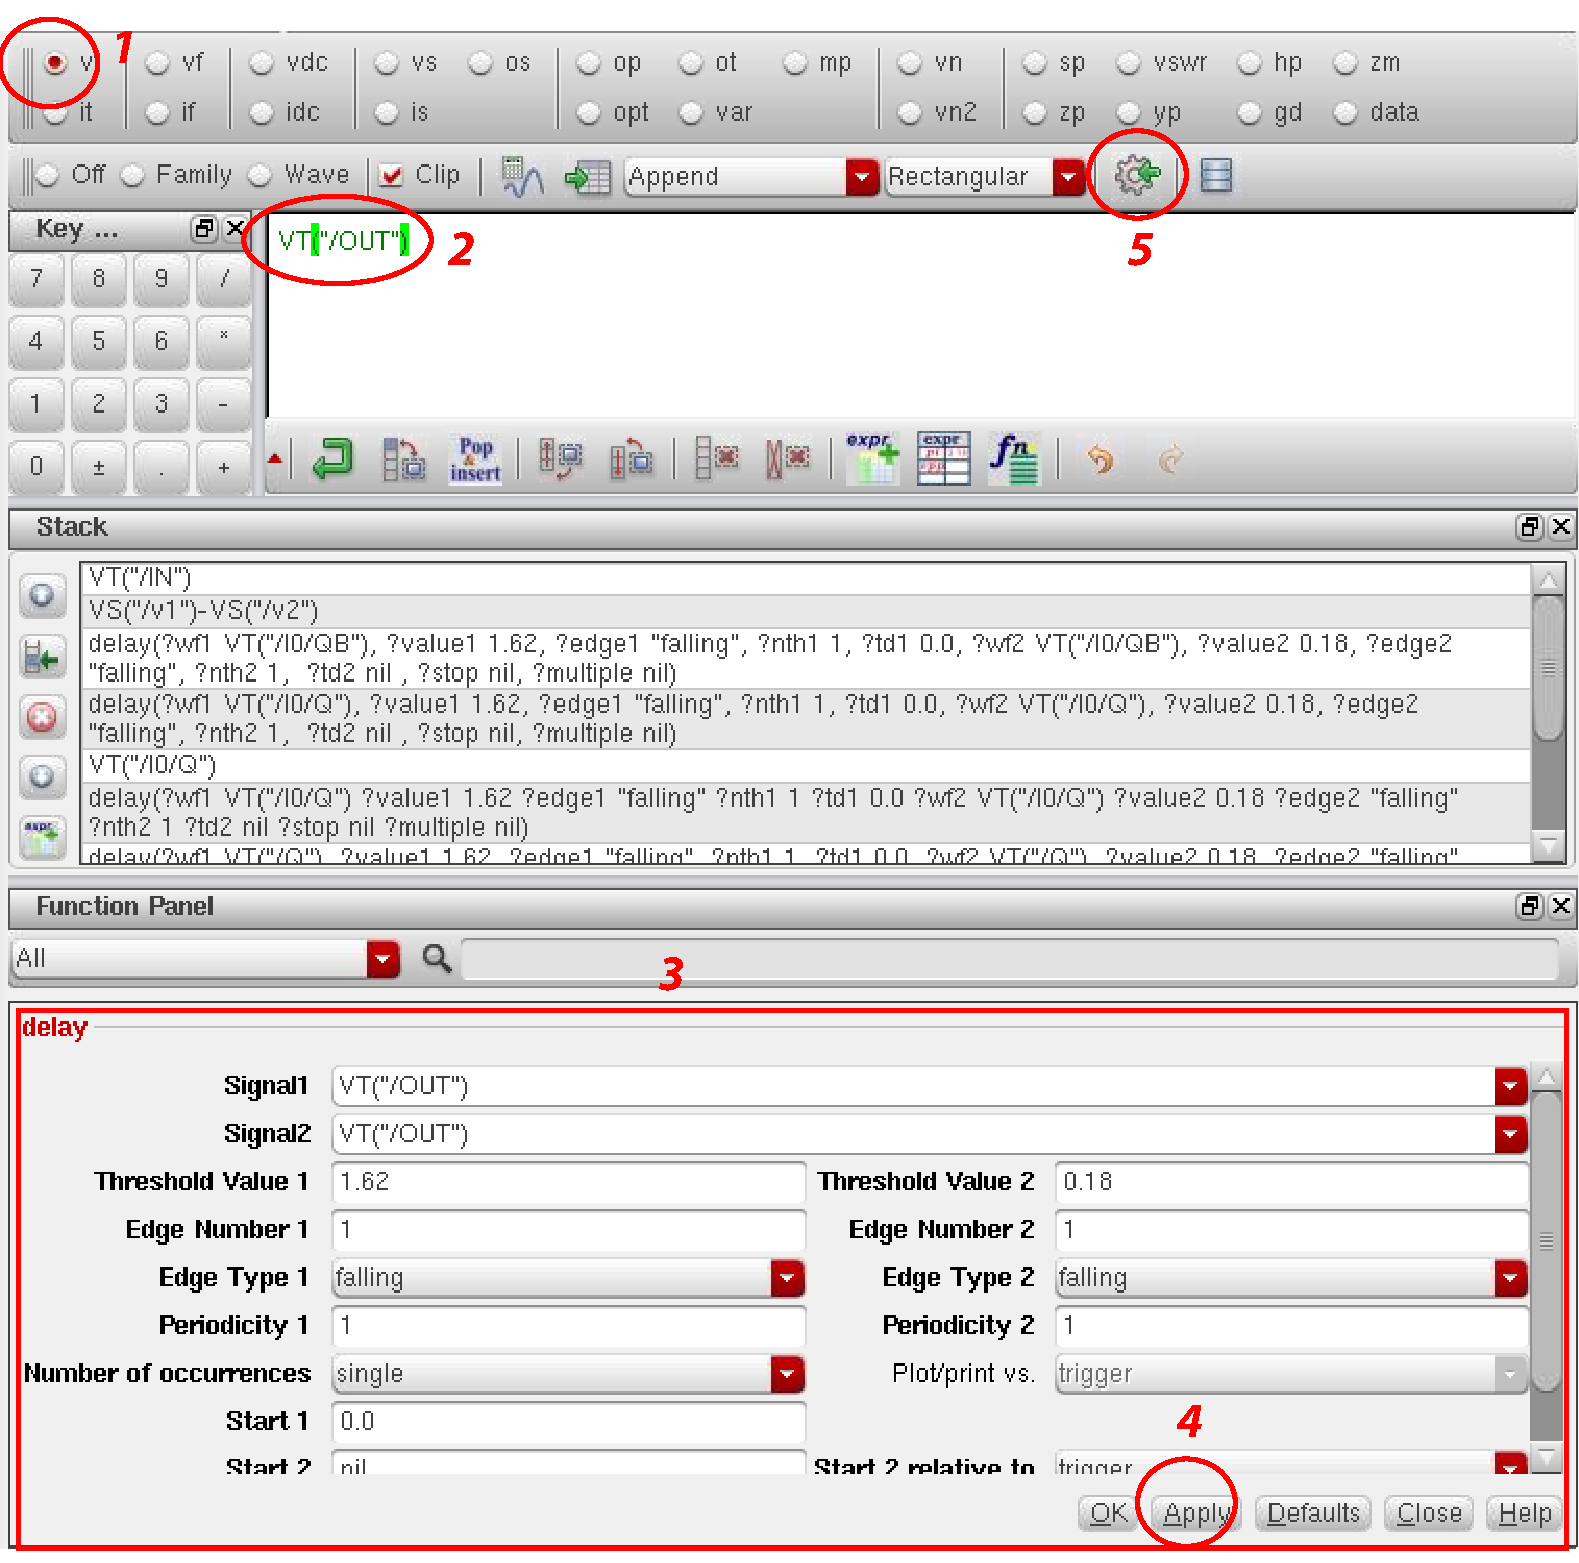
\includegraphics[scale=0.33]{figures/lab1_schematic_sim/calculator.pdf}
				\caption{ADE calculator setup.}
				\label{calculator}
			\end{wrapfigure}
			\item In the function panel, search for \textit{delay}.
			\item Select the appropriate signal you want to measure from (in this case, we want to measure the rising and falling time so select the output signal of your inverter): click on \textbf{vt} and select the signal on the schematic (step 1 in Fig. \ref{calculator}).
			\item Copy/paste the name of the signal in the Signal 1 and signal 2 fields of the calculator (step 2 in Fig. \ref{calculator}). Here, signal 1 and signal 2 are the same since we are measuring the falling delay which is on a single signal.
			\item Specify the other fields as in the picture (step 3 in Fig. \ref{calculator}). In this example, we show how to measure the falling delay (although the rising delay is obtained similarly). Threshold Value 1 is the value for which the time will be measured for the first point. If you want to measure the falling delay, it is $90\%$ of $V_{DD}$ so 1.62V. In the same manner, Threshold Value 2 is the value for which the time will be measured for the second point, so it is $10\%$ of $V_{DD}$ so 0.18V. Both Edge Types are falling since you are measuring a falling delay.		
					\item Click on \textit{Apply} (step 4).
			\item Finally, send the expression the ADE outputs (step 5). If you go back to the ADE window, the expression should be in the display output panel. Right click on it and select \textit{Edit} and change the \textit{Name (opt.)} field to an appropriate name (e.g. \textit{falling delay}).
			\item Redo the previous steps for the rising delay and the propagation delays. For the rising delay, note that both edges should be rising and the Threshold Values should be changed appropriately. For the propagation delay, don't forget to change Signal1 and Signal2 (this time, you are measuring a delay between the input and the output and not a delay on a single signal). Also, don't forget to carefully choose the threshold values (50$\%$) and the appropriate edge types.
		}
		
	\end{itemize}

\end{enumerate}

\begin{checkpoint}\label{check3}
	Please call an assistant and show him that you obtained the transient curve for your inverter successfully.
\end{checkpoint}	
\clearpage



\begin{exercise}\ \label{ex5}
	\vspace{-5mm}
	\begin{enumerate}
		\item Report the curve of the input/output of your inverter and the rising and falling times. Which one is faster? Why?
		\item Report the propagation delay of your inverter. How could you optimize it? At which cost?
		\item We considered a period time of 2ns. Is it slow, fast or appropriate compared to the frequency time of chips based on the 130$nm$ process? Justify your answer.			
	\end{enumerate}
\vspace{-5mm}
\end{exercise}


\subsection{Transient Simulation Under Different Process Corners}	
In VLSI design, corner simulations are used to represent the extreme cases of fabrication parameter variation and/or variation of other physical parameters such as the supply voltage or the temperature. When fabricated, depending on the fabrication process variations, devices may exhibit different behavior and therefore be faster, slower, larger, smaller and hence vary from the ideal case. As a result, the circuit may fall below the specifications. Corner simulations allow to model these cases and ensure that the circuit will still be functional under those variations. For your previous simulations, you used some model libraries in the \textit{tt} corner (typical $nmos$ - typical $pmos$) which are describing the characteristics (delay and power consumption mainly) of the transistors, diodes, \textit{etc.} under typical parameters. In this section, you will study the effect of the \textit{ss} (slow $nmos$ - slow $pmos$) and \textit{ff} (fast $nmos$ - fast $pmos$) corners on your design. To do so:	

\begin{itemize}
	\item From the ADE L window, click on \textit{Setup -> Model Libraries} as shown in Fig. \ref{fig_corner}.
	\item In the section column, find \textit{tt$\_$fet}, click on time on it, then a second time and change it to \textit{ff$\_$fet}.
	\item Run the simulation again and observe how the timing change.
	\item Repeat the process for the \textit{ss$\_$fet} corner.
	\begin{figure}[!h]
		\centering
		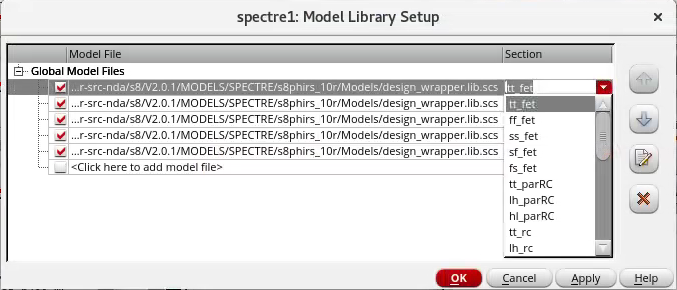
\includegraphics[scale=0.35]{figures/lab1_schematic_sim/tt}
		\caption{Changing the model library file corner.}
		\label{fig_corner}
	\end{figure}	
\end{itemize}

\begin{exercise}\ \label{ex6}
	\vspace{-5mm}
	\begin{enumerate}
			\item Report the rising and falling delays of your inverter for the \textit{ff} and \textit{ss} corners. How different are they from the \textit{tt} corner you used previously in the lab?
		\item After running some process corner simulations, if your inverter were to fall below a delay constraint, what could be done in order to make it faster and meet the constraint?
	\end{enumerate}
	\vspace{-5mm}
\end{exercise}

%process corner:
%Do with TT and SS
%what is the new delay? Why? If you had a timing constrain of XXX and it were failing for the SS corner, what could you do to ensure that your inv passes the specifications even for SS corner?

\section{Assignment and Checkpoint Summary}
Write a report and answer the assignments asked during the lab, which are summarized below. Do not forget to validate the checkpoints, summarized below as well, by an assistant before the end of the lab.


	\begin{exercisesum}\	
			\vspace{-2mm}
	\begin{enumerate}
		\item Report the I-V curves under different $VGS$ voltages for your \textit {nmos} transistor.
		\item What are the $I_{on}$, $I_{off}$ of your $nmos$ transistor? Remember that $I_{on}$ is the maximum achievable current and $I_{off}$ if the current when $VDS$ is set to the supply voltage but when the gate is off ($V_{GS}=0V$).
		\item Report the I-V curves under different $VGS$ voltages for your \textit {pmos} transistor as well as its $I_{on}$, $I_{off}$.
		\item Plot the Voltage Transfer Curve (VTC), report the switching point of the inverter and specify the dimensions of your transistors.
		\item Plot the VTC curve for different width of the \textit{pmos}. What is this effect called? Report for which value of the \textit{pmos} width the switching point is equal to $V_{DD}/2$.
		\item Report the curve of the input/output of your inverter and the rising and falling times. Which one is faster? Why?
	\item Report the propagation delay of your inverter. How could you optimize it? At which cost?
	\item We considered a period time of 2ns. Is it slow, fast or appropriate compared to the frequency time of chips based on the 130$nm$ process? Justify your answer.			
			\item Report the rising and falling delays of your inverter for the \textit{ff} and \textit{ss} corners. How different are they from the \textit{tt} corner you used previously in the lab?
	\item After running some process corner simulations, if your inverter were to fall below a delay constraint, what could be done in order to make it faster and meet the constraint?
	\end{enumerate}
\vspace{-5mm}
\end{exercisesum}	

\begin{checkpointsum}\
	\vspace{-2mm}
	\begin{enumerate}
		\item Please call an assistant and show him that you obtained the I-V curves for different $VGS$ for your $nmos$ successfully.
		\item Please call an assistant and show him that you obtained the VTC curve for your inverter successfully.
		\item Please call an assistant and show him that you obtained the transient curve for your inverter successfully.
	\end{enumerate}
	\vspace{-5mm}
\end{checkpointsum}